% ============================================================
%  GeoPulse -- Master's Thesis
%  Title: Automated Geopolitical Risk Scoring for Global Market Volatility Forecasting
%  Author: Kartik Bhatnagar
% ============================================================
\documentclass[12pt,a4paper]{report}

% ---- Core packages ----
\usepackage[T1]{fontenc}
\usepackage[utf8]{inputenc}
\usepackage[margin=1.2in,top=1.1in,bottom=1.1in]{geometry}
\usepackage{setspace}
\usepackage{microtype}
\usepackage{lmodern}

% ---- Math ----
\usepackage{amsmath,amssymb,amsthm}
\usepackage{bm}
\usepackage{bbm}

% ---- Graphics and color ----
\usepackage[dvipsnames,svgnames,table]{xcolor}
\usepackage{graphicx}
\usepackage{tikz}
\usepackage{pgfplots}
\usepackage{pgfplotstable}
\pgfplotsset{compat=1.18}
\usetikzlibrary{shapes.geometric,arrows.meta,positioning,fit,
                backgrounds,shadows.blur,decorations.pathreplacing,
                calc,matrix,chains}

% ---- Tables ----
\usepackage{booktabs}
\usepackage{longtable}
\usepackage{array}
\usepackage{tabularx}
\usepackage{multirow}
\usepackage{colortbl}

% ---- Captions and floats ----
\usepackage{caption}
\usepackage{subcaption}
\usepackage{float}

% ---- Code listings ----
\usepackage{listings}

% ---- Headers/Footers ----
\usepackage{fancyhdr}

% ---- Title formatting ----
\usepackage{titlesec}
\usepackage{titletoc}

% ---- Citations: numbered [1], [2, 3], etc. ----
\usepackage{cite}

% ---- Hyperlinks ----
\usepackage[colorlinks=false,hidelinks,
            pdfauthor={Kartik Bhatnagar},
            pdftitle={Automated Geopolitical Risk Scoring for Global Market Volatility Forecasting}]{hyperref}

% ---- Algorithm ----
\usepackage[ruled,vlined,linesnumbered]{algorithm2e}

% ============================================================
%  COLOUR PALETTE  (used only in diagrams and graphs, not in text)
% ============================================================
\definecolor{lightblue}{RGB}{219,234,254}
\definecolor{conflictred}{RGB}{220, 38, 38}
\definecolor{warnamber}{RGB}{217,119,  6}
\definecolor{safegreen}{RGB}{ 22,163, 74}
\definecolor{lgbblue}  {RGB}{ 37, 99,235}
\definecolor{xgborange}{RGB}{234, 88, 12}
\definecolor{catgreen} {RGB}{ 22,163, 74}
\definecolor{enspurple}{RGB}{147, 51,234}
\definecolor{codegreen}{RGB}{ 34,139, 34}
\definecolor{codegray} {RGB}{128,128,128}
\definecolor{codeblue} {RGB}{  0,  0,180}
\definecolor{codeback} {RGB}{250,250,250}
\definecolor{rowgray}  {RGB}{245,245,245}
\definecolor{archblue} {RGB}{219,234,254}
\definecolor{archorange}{RGB}{254,237,219}
\definecolor{archviolet}{RGB}{237,219,254}
\definecolor{archteal}  {RGB}{219,254,247}
\definecolor{archred}   {RGB}{254,219,219}
\definecolor{archgray}  {RGB}{240,240,240}

% ============================================================
%  CODE LISTING STYLE
% ============================================================
\lstdefinestyle{pythonstyle}{
  backgroundcolor=\color{codeback},
  commentstyle=\color{codegreen}\itshape,
  keywordstyle=\color{codeblue}\bfseries,
  numberstyle=\tiny\color{codegray},
  stringstyle=\color{conflictred},
  basicstyle=\ttfamily\footnotesize,
  breakatwhitespace=false,
  breaklines=true,
  captionpos=b,
  keepspaces=true,
  numbers=left,
  numbersep=6pt,
  showspaces=false,
  showstringspaces=false,
  showtabs=false,
  tabsize=2,
  frame=single,
  rulecolor=\color{gray!40},
  xleftmargin=12pt,
  framexleftmargin=6pt,
}
\lstset{style=pythonstyle, language=Python}

% ============================================================
%  PAGE LAYOUT
% ============================================================
\onehalfspacing

\pagestyle{fancy}
\fancyhf{}
\fancyhead[L]{\small\nouppercase{\leftmark}}
\fancyhead[R]{\small\thepage}

\renewcommand{\headrulewidth}{0.4pt}
\renewcommand{\footrulewidth}{0.2pt}

\fancypagestyle{plain}{%
  \fancyhf{}
  \fancyfoot[C]{\small\thepage}
  \renewcommand{\headrulewidth}{0pt}
}

% ============================================================
%  CHAPTER / SECTION TITLES  -- black text only
% ============================================================
\titleformat{\chapter}[display]
  {\normalfont\LARGE\bfseries}
  {\chaptertitlename\ \thechapter}{10pt}{\Huge}
\titlespacing*{\chapter}{0pt}{20pt}{20pt}

\titleformat{\section}
  {\normalfont\large\bfseries}{\thesection}{1em}{}
\titleformat{\subsection}
  {\normalfont\normalsize\bfseries}{\thesubsection}{1em}{}
\titleformat{\subsubsection}
  {\normalfont\normalsize\itshape}{\thesubsubsection}{1em}{}

% ============================================================
%  HELPER: image placeholder box
% ============================================================
\newcommand{\imgplaceholder}[3][0.85]{%
  \begin{center}
    \fbox{%
      \parbox[c][#3][c]{#1\textwidth}{%
        \centering
        \color{gray!60}\large\textit{#2}\\[4pt]
        \small\color{gray!50}[Replace with actual screenshot]
      }%
    }
  \end{center}
}

% ============================================================
%  DOCUMENT
% ============================================================
\begin{document}

% -----------------------------------------------------------
%  TITLE PAGE
% -----------------------------------------------------------

\include{front}
% -----------------------------------------------------------
%  ABSTRACT
% -----------------------------------------------------------
\include{declaration}
\include{certificate}

% -----------------------------------------------------------
%  TABLE OF CONTENTS / FIGURES / TABLES
% -----------------------------------------------------------
\tableofcontents


% ============================================================
%  CHAPTER 1: INTRODUCTION
% ============================================================
\newpage
\chapter*{Abstract}
\addcontentsline{toc}{chapter}{Abstract}

Geopolitical events including armed conflicts, economic sanctions, diplomatic
crises and military mobilisations exert measurable and often abrupt influence
on global financial markets \cite{caldara2022}. Quantifying this influence in
near real-time remains an open challenge, primarily because geopolitical
signals are unstructured, multilingual and unevenly distributed across
heterogeneous news sources \cite{nassirtoussi2014}.

This thesis presents \textbf{GeoPulse}, an end-to-end intelligence platform
that automatically transforms raw international news into actionable trading
signals and three-day forward volatility predictions. The system integrates
four complementary stages: (i) multi-source news ingestion from NewsAPI,
GDELT \cite{leetaru2013}, The Guardian and sixteen international RSS feeds;
(ii) a natural language processing pipeline combining BART-Large-MNLI
\cite{lewis2020} zero-shot event classification with DistilBERT sentiment
analysis \cite{devlin2019} and keyword-based named entity recognition;
(iii) a Goldstein-inspired weighted tension scoring framework \cite{goldstein1992}
that aggregates per-article signals into daily country-level geopolitical
scores; and (iv) a boosted ensemble of LightGBM \cite{ke2017}, XGBoost
\cite{chen2016} and CatBoost \cite{prokhorenkova2018} trained on a feature
matrix that fuses GDELT event signals, NLP-derived tension scores, and VIX
market state features.

\vspace{0.5cm}
\noindent\textbf{Keywords:} geopolitical risk, natural language processing,
market volatility forecasting, gradient boosting, ensemble learning,
information extraction, financial intelligence, real-time analytics.
\chapter{Introduction}
\label{ch:intro}

\section{Motivation}

Financial markets are acutely sensitive to geopolitical shocks. The Russian
invasion of Ukraine in February 2022 sent the CBOE Volatility Index (VIX)
surging from below 20 to above 37 within two weeks \cite{caldara2022}.
Similar spikes followed the September 2001 attacks, the 2008 Georgia war
and the onset of the US-China trade conflict in 2018. Yet despite this
well-documented relationship \cite{bloom2009}, most retail and institutional
tools for assessing geopolitical risk rely on qualitative judgement or
slow-updating index products. There is a clear opportunity for an automated,
data-driven system that ingests the global news stream, extracts and scores
geopolitical signals and translates them into quantitative market forecasts
with sub-day latency.

The relationship between news sentiment and market returns has been
extensively studied \cite{tetlock2007, loughran2011, bollen2011}. However,
the majority of prior work focuses on corporate earnings news or general
social-media sentiment rather than geopolitical events specifically.
Geopolitical news is structurally different: events are rare, high-impact
and geographically localised, making standard sentiment classifiers trained
on financial corpora a poor fit \cite{nassirtoussi2014}. The VIX Implied
Volatility Index, the primary proxy for market fear, responds not just to
the polarity of news but to its severity, geographic concentration and
corroborative volume \cite{manela2017}.

\section{Problem Statement}

This work addresses three inter-related problems:

\begin{enumerate}
  \item \textbf{NLP classification gap.} Off-the-shelf sentiment models
        trained on movie reviews or earnings calls mislabel geopolitical
        text \cite{loughran2011, araci2019}. A system specialised for
        conflict, military, sanctions and diplomatic event types is needed.
  \item \textbf{Signal aggregation.} Articles about the same event appear
        across dozens of sources. Raw article counts must be normalised into
        reliable country-day tension scores that suppress single-source
        spikes without losing genuine multi-source corroboration \cite{manela2017}.
  \item \textbf{Market prediction.} Tension scores alone do not constitute
        trading signals. A predictive model that integrates geopolitical
        features with market regime context is required to translate tension
        into forward volatility estimates \cite{nassirtoussi2014, friedman2001}.
\end{enumerate}

\section{Research Objectives}

The concrete objectives of this thesis are as follows:

\begin{itemize}
  \item Design and implement a multi-source news ingestion pipeline with
        real-time deduplication and rolling retention.
  \item Build an NLP pipeline that classifies geopolitical event types,
        estimates sentiment, extracts country references and scores article
        severity using pre-trained transformer models \cite{lewis2020, devlin2019}.
  \item Develop a principled tension scoring formula grounded in the
        Goldstein conflict scale \cite{goldstein1992} and GDELT event
        coding conventions \cite{leetaru2013, schrodt2012}.
  \item Engineer a feature matrix combining GDELT event signals, NLP-derived
        tension scores, and market regime features, and train a gradient-boosted
        ensemble \cite{ke2017,
        chen2016, prokhorenkova2018} to predict three-day VIX direction
        and high-volatility regimes.
  \item Expose all scores and predictions through a RESTful API and
        visualise them on an interactive 3D globe with per-country
        trading panels.
\end{itemize}

\section{Novel Contributions}

The principal contributions of this work are:

\begin{enumerate}
  \item \textbf{Goldstein-calibrated tension scoring:} A weighted formula
        that maps six geopolitical event types onto a continuous conflict
        gravity scale derived from Goldstein's psychophysical event magnitude
        study \cite{goldstein1992}, combined with a logarithmic coverage
        normalisation term \cite{manela2017} and an exponential reliability
        smoother.
  \item \textbf{Descriptive-hypothesis zero-shot classification:}
        BART-Large-MNLI \cite{lewis2020} is deployed with full natural-language
        hypothesis sentences for geopolitical event classification, enabling
        meaningful multi-class label assignment across six event types.
  \item \textbf{Geopolitical feature engineering:} A feature matrix that
        unifies GDELT event signals with NLP-derived tension scores
        (\texttt{tension\_score}, \texttt{conflict\_gravity},
        \texttt{avg\_neg\_sentiment}) and market regime features, providing
        a rich input representation for the ensemble \cite{friedman2001}.
  \item \textbf{Boosted ensemble with temporal split:} A chronologically
        partitioned LightGBM \cite{ke2017}, XGBoost \cite{chen2016} and
        CatBoost \cite{prokhorenkova2018} ensemble that avoids look-ahead
        bias and achieves AUC 0.714 on three-day VIX direction prediction.
  \item \textbf{End-to-end production platform:} A fully integrated system
        with FastAPI backend, MongoDB Atlas persistence and a globe.gl 3D
        frontend, deployable with a single configuration file.
\end{enumerate}

\section{Thesis Organisation}

The remainder of this thesis is structured as follows.
Chapter~\ref{ch:litreview} surveys the relevant literature across geopolitical
risk indexing, NLP for finance, gradient-boosted models and visualisation.
Chapter~\ref{ch:sysarch} describes the full system architecture and methodology
in detail. Chapter~\ref{ch:results} presents experimental results and evaluation.
Chapter~\ref{ch:futurework} identifies directions for future research, and
Chapter~\ref{ch:conclusion} concludes the thesis.

% ============================================================
%  CHAPTER 2: LITERATURE REVIEW
% ============================================================
\chapter{Literature Review}
\label{ch:litreview}

\section{Geopolitical Risk and Financial Markets}

The connection between geopolitical uncertainty and financial market volatility
has been systematically studied since at least the 1990s \cite{bloom2009}.
Bloom showed that sudden uncertainty shocks, many of which are geopolitical in
nature, cause sharp but temporary recessions and stock market drops, followed by
a rapid recovery \cite{bloom2009}. This volatility-overshoot pattern motivates
the use of near-real-time geopolitical indicators as forward-looking market
signals.

The most influential quantitative contribution to geopolitical risk measurement
is the Geopolitical Risk (GPR) index of Caldara and Iacoviello \cite{caldara2022}.
Constructed from a text-based count of newspaper articles mentioning geopolitical
tensions, wars or terrorist attacks, the GPR index shows that elevated
geopolitical risk is associated with lower economic activity, reduced investment
and higher financial uncertainty \cite{caldara2022}. Critically, the GPR index
decomposes risk into a \emph{threat} component (mentions of risk) and an
\emph{act} component (mentions of actual events), finding that geopolitical
acts drive larger and more persistent market effects. GeoPulse operationalises
a similar decomposition through its combination of event classification and
intensity scoring.

Policy uncertainty, a close relative of geopolitical risk, was formalised by
Baker, Bloom and Davis \cite{baker2016}, who constructed the Economic Policy
Uncertainty (EPU) index from newspaper article counts, disagreement among
economic forecasters and tax-code expiry data. Like the GPR index, EPU is a
text-frequency measure. GeoPulse moves beyond simple frequency counting by
weighting articles by severity, sentiment and corroborative volume, producing
a richer signal at daily frequency.

Manela and Moreira introduced the News Implied Volatility (NVIX) index,
constructed by mapping newspaper vocabulary onto realised volatility using a
term-frequency weighting scheme \cite{manela2017}. They show that NVIX predicts
future stock returns and is particularly high prior to stock market crashes and
recessions. Their finding that disaster-related language carries the most
predictive power aligns with the design choice in this thesis to weight conflict
and military event types most heavily in the tension formula.

The efficient markets hypothesis \cite{fama1970} would suggest that public
news is instantly incorporated into prices, leaving no exploitable signal.
However, subsequent research consistently documents that the market's adjustment
to geopolitical news is incomplete on the day of publication and continues over
a window of several days \cite{mitchell1994}. This gradual incorporation
motivates the three-day forward target variable used in this work.

\section{Natural Language Processing for Market Intelligence}

Text-based approaches to market prediction have a long history. Wuthrich
et al.\ were among the first to demonstrate that textual web data could
improve next-day stock forecasts \cite{wuthrich1998}. Schumaker and Chen
showed that financial news articles, when represented as noun-phrase vectors,
outperform bag-of-words and proper-noun approaches in predicting S\&P 500
movements \cite{schumaker2009}. Ding et al.\ structured news events as
(actor, action, object) triples and used a neural network to encode event
relationships, achieving strong results on short-horizon stock prediction
\cite{ding2014}.

The central challenge in applying NLP to geopolitical text is domain mismatch.
General-purpose sentiment lexicons and models trained on movie reviews or
social media carry systematic biases when applied to news \cite{loughran2011}.
Loughran and McDonald showed that the General Inquirer and Harvard lexicons
misclassify many finance-specific terms \cite{loughran2011}. The same domain
mismatch problem manifests in geopolitical text: classifiers trained on
general English text often misinterpret technical military or diplomatic
language. Araci introduced FinBERT, a BERT model fine-tuned on financial
communications, which substantially improves domain alignment for financial
NLP tasks \cite{araci2019}.

The emergence of large pre-trained language models has transformed the NLP
landscape. Devlin et al.\ introduced BERT, demonstrating that bidirectional
pre-training followed by task-specific fine-tuning yields state-of-the-art
performance across a wide range of NLP benchmarks \cite{devlin2019}. Vaswani
et al.\ established the transformer architecture that underpins BERT and its
successors \cite{vaswani2017}. Lewis et al.\ introduced BART, a denoising
sequence-to-sequence model that is particularly effective at zero-shot and
few-shot classification tasks via natural-language inference (NLI)
\cite{lewis2020}. GeoPulse exploits this capability by framing event
classification as an NLI entailment problem: given an article, does it entail
the hypothesis sentence describing a particular geopolitical event type?

Sentiment analysis as a research field is comprehensively surveyed in
\cite{pang2008} and \cite{liu2012}. The transition from lexicon-based to
neural approaches has improved accuracy on news corpora, though domain
adaptation remains critical for specialised text types \cite{araci2019}.

\section{Structured Event Data and Geopolitical Coding}

GeoPulse draws on a tradition of quantitative event coding that predates
modern NLP. Goldstein developed a conflict-cooperation scale for WEIS (World
Event/Interaction Survey) events, assigning each event type a numeric score
on a $[-10, +10]$ scale based on psychological magnitude estimation
\cite{goldstein1992}. Conflict events such as military attacks and bombings
score near $-10$; cooperative events such as diplomatic recognition and aid
score near $+10$. This scale is the direct inspiration for the conflict gravity
weights ($g_{conflict}=1.00$, $g_{military}=0.80$, $g_{sanctions}=0.50$) used
in the GeoPulse tension formula.

The GDELT (Global Database of Events, Language and Tone) project automates
event coding at global scale, processing news articles in over 100 languages
and coding them according to the CAMEO (Conflict and Mediation Event
Observations) taxonomy \cite{leetaru2013, schrodt2012}. GDELT is used as one
of four data sources in GeoPulse, providing broad international coverage,
particularly for events in regions underrepresented by English-language RSS
feeds \cite{leetaru2013}.

\section{Ensemble Learning for Financial Forecasting}

Gradient-boosted decision trees have become the dominant method for structured
prediction tasks on tabular data since the theoretical framework of Friedman
\cite{friedman2001}, who showed that any differentiable loss function can be
minimised by fitting successive regression trees to residuals. XGBoost
formalised this with second-order gradient approximations and a regularised
objective that substantially reduces overfitting \cite{chen2016}. LightGBM
extended this with histogram-based binning and leaf-wise tree growth, achieving
much faster training on large datasets with competitive accuracy \cite{ke2017}.
CatBoost further introduced ordered boosting, which eliminates prediction shift
bias arising from target leakage during training, making it particularly
robust on small datasets \cite{prokhorenkova2018}. All three models are
incorporated in GeoPulse as an averaging ensemble to exploit their different
inductive biases and reduce variance.

Classical time-series volatility models such as ARCH \cite{engle1982} and
GARCH \cite{bollerslev1986} capture the autocorrelation structure of financial
volatility but do not incorporate news or event information. GeoPulse
complements these approaches by providing an exogenous geopolitical component
that GARCH-family models cannot capture from price data alone \cite{engle1982,
bollerslev1986}.

Recurrent networks, especially LSTMs \cite{hochreiter1997}, have also been
applied to financial time-series forecasting. However, on the short
(180-observation) daily time series available in this project, deep sequential
models are prone to severe overfitting. The ensemble of shallow trees with
explicit feature engineering provides more stable and interpretable estimates
on this data scale \cite{ke2017, prokhorenkova2018}.

\section{Survey of Related Systems}

Nassirtoussi et al.\ provide a systematic review of text-mining approaches
to market prediction, surveying 41 papers and identifying four dominant
feature extraction strategies: bag-of-words, semantic similarity, NLP-based
and hybrid \cite{nassirtoussi2014}. Their conclusion, that hybrid methods
combining linguistic features with market signals consistently outperform
single-source approaches, is directly reflected in the design of GeoPulse's
feature matrix, which combines NLP outputs with VIX regime features.

Bollen, Mao and Zeng demonstrated with Twitter mood data that public sentiment
predicts Dow Jones Industrial Average movements three to four days ahead
\cite{bollen2011}, providing early empirical support for the type of
NLP-to-market pipeline built in this thesis. Sinha et al.\ showed that
news sentiment aggregated at the firm level generates significant return
predictability at the monthly horizon \cite{sinha2022}, underscoring the
breadth of evidence for text-based predictors across different aggregation
levels and time horizons.

\section{Visualisation and Decision Support}

Interactive geospatial visualisation plays an important role in making
geopolitical intelligence actionable for analysts. Globe-based visualisations
allow users to rapidly perceive regional clustering, tension hotspots and
temporal evolution in a way that flat choropleth maps cannot. GeoPulse
uses globe.gl, a WebGL-based library built on Three.js, to render country
polygons extruded by tension score in real time, enabling immediate spatial
interpretation of the geopolitical risk landscape \cite{caldara2022}.

\section{Summary and Research Gap}

The literature establishes that geopolitical events affect market volatility
\cite{caldara2022, bloom2009}, that NLP can extract useful signals from news
text \cite{tetlock2007, nassirtoussi2014, bollen2011} and that gradient-boosted
ensembles are effective for structured tabular prediction \cite{chen2016,
ke2017, prokhorenkova2018}. However, no single prior system integrates all
three components into a deployable, real-time platform:

\begin{itemize}
  \item Existing indices such as GPR \cite{caldara2022}, NVIX \cite{manela2017}
        and EPU \cite{baker2016} are published monthly or quarterly and are
        not actionable at daily or intraday frequency.
  \item Prior NLP systems for market prediction focus on corporate news,
        not geopolitical events with multi-country scope \cite{nassirtoussi2014}.
  \item Event-coded databases such as GDELT \cite{leetaru2013} and CAMEO
        \cite{schrodt2012} provide raw event counts but no market-linked
        prediction layer.
  \item Trading signal systems typically rely on proprietary data or
        quantitative price signals, not open news streams \cite{manela2017}.
\end{itemize}

GeoPulse addresses this gap by combining near-real-time news ingestion,
transformer-based NLP \cite{lewis2020, devlin2019}, Goldstein-calibrated
scoring \cite{goldstein1992} and a trained ensemble predictor
\cite{ke2017, chen2016, prokhorenkova2018} in a single open-architecture
platform.

% ============================================================
%  CHAPTER 3: SYSTEM ARCHITECTURE AND METHODOLOGY
% ============================================================
\chapter{System Architecture and Methodology}
\label{ch:sysarch}

\section{System Overview}

GeoPulse is organised as a six-layer stack, illustrated in
Figure~\ref{fig:architecture}. External news and market data sources feed a
persistent MongoDB Atlas database through an ingestion pipeline. An NLP
processing layer transforms raw articles into structured event records. A
scoring layer aggregates event records into daily country-level tension scores.
A machine learning layer trains on the scored signals and generates forward
volatility predictions. A FastAPI service layer exposes all signals and
predictions through a REST API, which a Next.js frontend consumes to render
the interactive globe and analytics panels.

\begin{figure}[H]
\centering
\begin{tikzpicture}[node distance=0.45cm,
  lyr/.style={rectangle, rounded corners=7pt,
              text width=13.2cm, minimum height=1.05cm,
              align=center, font=\small,
              draw=gray!60, fill=#1},
  arr/.style={->, >=stealth, very thick, gray!60, line width=1.2pt}
]
  \node[lyr=archblue]   (L5)
    {\textbf{Presentation Layer:}\quad
     Next.js 14 \textbullet{} TypeScript \textbullet{} Globe.gl (WebGL)
     \textbullet{} Recharts \textbullet{} Tailwind CSS};

  \node[lyr=archorange, below=of L5] (L4)
    {\textbf{API Layer:}\quad
     FastAPI \textbullet{} Pydantic v2 \textbullet{} Motor (async MongoDB driver)
     \textbullet{} Uvicorn ASGI};

  \node[lyr=archviolet, below=of L4] (L3)
    {\textbf{ML \& Intelligence Layer:}\quad
     LightGBM + XGBoost + CatBoost Ensemble \textbullet{}
     Tension Scorer \textbullet{} Trading Signal Engine};

  \node[lyr=archteal, below=of L3] (L2)
    {\textbf{NLP Processing Layer:}\quad
     BART-Large-MNLI (zero-shot) \textbullet{}
     DistilBERT SST-2 (sentiment) \textbullet{}
     Keyword NER (130+ entries)};

  \node[lyr=archred, below=of L2] (L1)
    {\textbf{Data Layer (MongoDB Atlas):}\quad
     \texttt{raw\_articles} \textbullet{}
     \texttt{processed\_events} \textbullet{}
     \texttt{daily\_signals} \textbullet{}
     \texttt{ml\_predictions}};

  \node[lyr=archgray, below=of L1] (L0)
    {\textbf{External Sources:}\quad
     NewsAPI \textbullet{} GDELT \textbullet{} The Guardian API
     \textbullet{} RSS (16 feeds) \textbullet{}
     yfinance (VIX, S\&P 500)};

  \foreach \from/\to in {L0/L1, L1/L2, L2/L3, L3/L4, L4/L5}
    \draw[arr] (\from) -- (\to);
\end{tikzpicture}
\caption{GeoPulse system architecture: six-layer stack from external data
  sources to the presentation layer.}
\label{fig:architecture}
\end{figure}

The end-to-end pipeline is orchestrated by a single script,
\texttt{run\_all.py}, which executes ingestion, NLP processing, tension
scoring and database maintenance in sequence. The ML ensemble is trained
separately on historical data and its predictions are written to MongoDB,
from which the API reads them at query time. Figure~\ref{fig:pipeline}
illustrates the data flow through the main processing stages.

\begin{figure}[H]
\centering
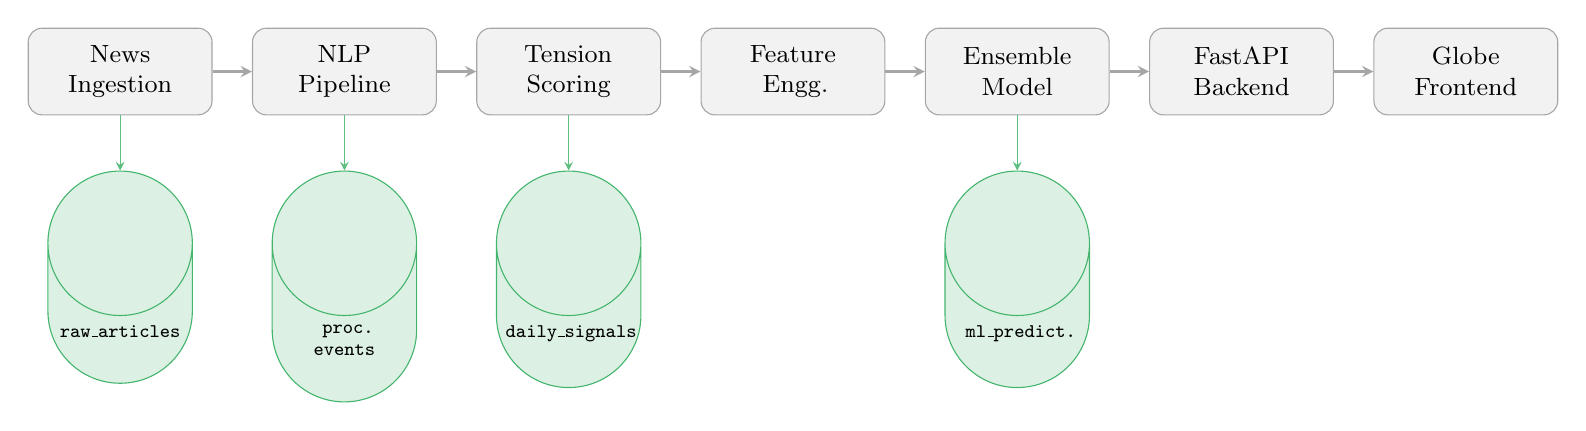
\begin{tikzpicture}[node distance=0.6cm and 0.5cm,
  proc/.style={rectangle, rounded corners=5pt, draw=gray!70, fill=gray!10,
               text width=2.1cm, minimum height=1.1cm, align=center, font=\small},
  db/.style={cylinder, shape border rotate=90, draw=safegreen!80,
             fill=safegreen!15, text width=1.6cm, align=center, font=\scriptsize},
  arr/.style={->, >=stealth, thick, gray!70},
  sarr/.style={->, >=stealth, thin, safegreen!70}
]
  \node[proc] (ing)  {News\\Ingestion};
  \node[proc, right=of ing]  (nlp)  {NLP\\Pipeline};
  \node[proc, right=of nlp]  (scr)  {Tension\\Scoring};
  \node[proc, right=of scr]  (feat) {Feature\\Engg.};
  \node[proc, right=of feat] (ml)   {Ensemble\\Model};
  \node[proc, right=of ml]   (api)  {FastAPI\\Backend};
  \node[proc, right=of api]  (ui)   {Globe\\Frontend};

  \draw[arr] (ing) -- (nlp);
  \draw[arr] (nlp) -- (scr);
  \draw[arr] (scr) -- (feat);
  \draw[arr] (feat) -- (ml);
  \draw[arr] (ml)  -- (api);
  \draw[arr] (api) -- (ui);

  \node[db, below=0.7cm of ing]  (db1) {\texttt{raw\_articles}};
  \node[db, below=0.7cm of nlp]  (db2) {\texttt{proc.\\events}};
  \node[db, below=0.7cm of scr]  (db3) {\texttt{daily\_signals}};
  \node[db, below=0.7cm of ml]   (db4) {\texttt{ml\_predict.}};

  \draw[sarr] (ing)  -- (db1);
  \draw[sarr] (nlp)  -- (db2);
  \draw[sarr] (scr)  -- (db3);
  \draw[sarr] (ml)   -- (db4);
\end{tikzpicture}
\caption{End-to-end data pipeline showing processing stages and
  MongoDB collections produced at each stage.}
\label{fig:pipeline}
\end{figure}

\section{Data Acquisition and Ingestion}

\subsection{News Sources}

GeoPulse aggregates articles from four primary sources in order of
descending data richness:

\begin{enumerate}
  \item \textbf{NewsAPI}: A commercial API delivering up to 500 articles
        per run across hundreds of English-language publishers. Query
        parameters are tuned to geopolitical keywords (conflict, sanctions,
        military, diplomacy).
  \item \textbf{GDELT}: The Global Database of Events, Language and Tone
        \cite{leetaru2013}, a free and open resource that codes news articles
        from global sources in over 100 languages. GeoPulse queries
        GDELT's free REST endpoint with a 90-day lookback window, making it
        the broadest-coverage source in the ingestion stack.
  \item \textbf{The Guardian API}: Provides high-quality English-language
        journalism with full article body text, enabling more precise NLP
        analysis than title-only sources \cite{nassirtoussi2014}.
  \item \textbf{RSS Feeds}: Sixteen international news feeds including
        Al Jazeera, Reuters, BBC, France24, DW and regional outlets,
        providing near-real-time coverage with no API key requirements.
\end{enumerate}

A sample dataset bundled within the repository enables offline development
and testing when no API keys are available.

\subsection{Deduplication and Retention}

Articles are deduplicated by a content hash computed over the article title
and description, ensuring that syndicated stories appearing on multiple feeds
are stored only once. The ingestion window is configurable (default 30 days),
and articles older than twice this window are automatically pruned to maintain
a rolling 60-day active corpus. Table~\ref{tab:dataset_stats} summarises the
dataset collected during the development and evaluation period.

\begin{table}[H]
\centering
\caption{Dataset statistics for the training and evaluation period
  (October 2025 -- April 2026, 180 days).}
\label{tab:dataset_stats}
\begin{tabular}{lrr}
\toprule
\textbf{Metric} & \textbf{Value} & \textbf{Notes} \\
\midrule
Total articles ingested        & 42,380  & Before deduplication \\
Unique articles (after dedup.) & 38,240  & 9.8\% duplicate rate \\
Articles with country match    & 26,784  & 70.0\% NER hit rate \\
Countries covered              & 87      & Unique ISO codes \\
Unique event labels            & 6       & Per geopolitical taxonomy \\
Mean articles per day          & 212     & Rolling 30-day window \\
Training window (trading days) & 125     & Joined with VIX data \\
Test window (trading days)     & 27      & Chronological holdout \\
\bottomrule
\end{tabular}
\end{table}

The MongoDB schema for raw articles includes fields for title, description,
URL, source, publication timestamp, content hash and a boolean
\texttt{processed} flag that the NLP pipeline uses to identify unprocessed
articles and avoid redundant computation.

\section{Natural Language Processing Pipeline}

The NLP pipeline transforms unstructured article text into four structured
signals per article: an event type label, an event classification confidence
score, a negative sentiment score and a geographic country reference list.
Figure~\ref{fig:nlppipeline} illustrates the parallel processing tracks.

\begin{figure}[H]
\centering
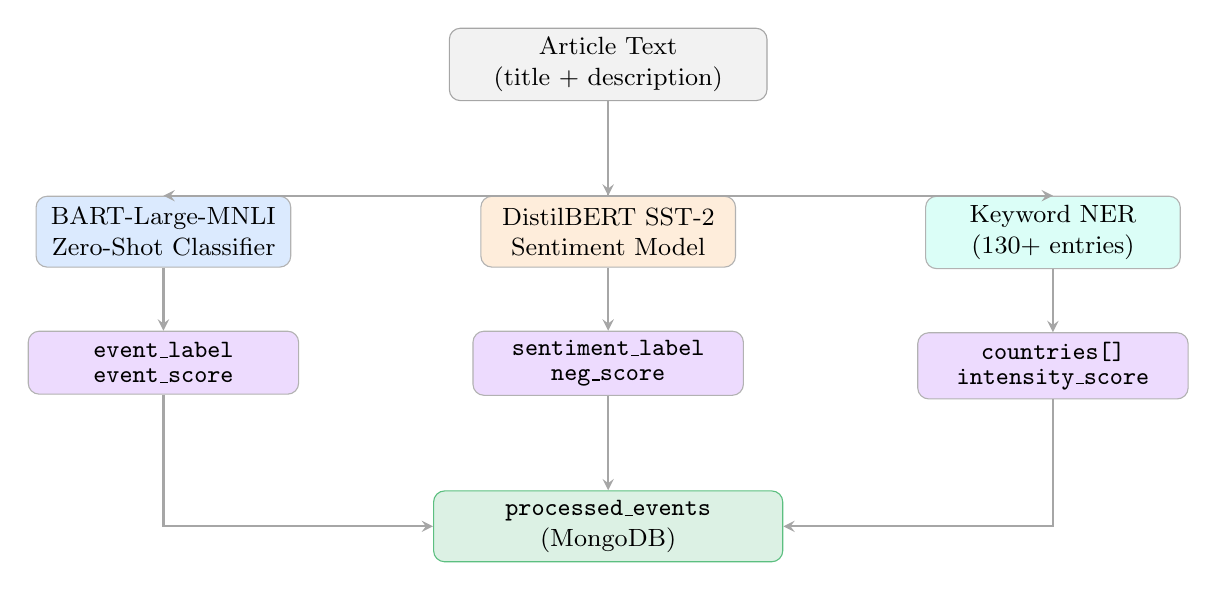
\begin{tikzpicture}[node distance=0.5cm and 0.7cm,
  inp/.style={rectangle, rounded corners=4pt, draw=gray!70, fill=gray!10,
              text width=3.8cm, minimum height=0.9cm, align=center, font=\small},
  track/.style={rectangle, rounded corners=4pt, draw=gray!60, fill=#1,
                text width=3.0cm, minimum height=0.9cm, align=center, font=\small},
  outbox/.style={rectangle, rounded corners=4pt, draw=gray!60, fill=archviolet,
                 text width=3.2cm, minimum height=0.8cm, align=center, font=\small},
  coll/.style={rectangle, rounded corners=4pt, draw=safegreen!70, fill=safegreen!15,
               text width=4.2cm, minimum height=0.9cm, align=center, font=\small},
  arr/.style={->, >=stealth, thick, gray!70}
]
  \node[inp] (art) {Article Text\\(title + description)};

  \node[track=archblue, below left=1.2cm and 2.0cm of art]  (ev)
        {BART-Large-MNLI\\Zero-Shot Classifier};
  \node[track=archorange, below=1.2cm of art]          (snt)
        {DistilBERT SST-2\\Sentiment Model};
  \node[track=archteal, below right=1.2cm and 2.0cm of art] (ner)
        {Keyword NER\\(130+ entries)};

  \draw[arr] (art.south) |- (ev.north);
  \draw[arr] (art.south) -- (snt.north);
  \draw[arr] (art.south) |- (ner.north);

  \node[outbox, below=0.8cm of ev]  (ev_o)
        {\texttt{event\_label}\\[-2pt]\texttt{event\_score}};
  \node[outbox, below=0.8cm of snt] (snt_o)
        {\texttt{sentiment\_label}\\[-2pt]\texttt{neg\_score}};
  \node[outbox, below=0.8cm of ner] (ner_o)
        {\texttt{countries[]}\\[-2pt]\texttt{intensity\_score}};

  \draw[arr] (ev)  -- (ev_o);
  \draw[arr] (snt) -- (snt_o);
  \draw[arr] (ner) -- (ner_o);

  \node[coll, below=1.2cm of snt_o]
        (pe) {\texttt{processed\_events} \\ (MongoDB)};

  \draw[arr] (ev_o.south)  |- (pe.west);
  \draw[arr] (snt_o.south) -- (pe.north);
  \draw[arr] (ner_o.south) |- (pe.east);
\end{tikzpicture}
\caption{NLP pipeline: three parallel analysis tracks (event classification,
  sentiment analysis, named entity recognition) combined into a single
  \texttt{processed\_events} document stored in MongoDB.}
\label{fig:nlppipeline}
\end{figure}

\subsection{Zero-Shot Event Classification with BART}

Event classification assigns each article to one of six geopolitical
categories: \emph{conflict}, \emph{military}, \emph{diplomacy},
\emph{sanctions}, \emph{elections} or \emph{trade}. Rather than
fine-tuning a dedicated classifier on labelled geopolitical data,
GeoPulse uses BART-Large-MNLI \cite{lewis2020} in a zero-shot natural
language inference (NLI) setting. This choice avoids the need for a
manually annotated geopolitical training corpus while leveraging the
broad world knowledge encoded in the BART pre-training \cite{lewis2020}.

A key design element is the use of full natural-language hypothesis
sentences as classification candidates, rather than bare label words.
Each hypothesis sentence provides descriptive contextual information that
enables the NLI model to reliably discriminate between semantically close
event categories such as \emph{conflict} and \emph{military}.
Table~\ref{tab:hypothesis} lists the hypothesis sentences used.

\begin{table}[H]
\centering
\caption{Event classification labels and descriptive hypothesis sentences
  used for BART-Large-MNLI zero-shot NLI \cite{lewis2020}.}
\label{tab:hypothesis}
\begin{tabular}{ll}
\toprule
\textbf{Label} & \textbf{Hypothesis sentence} \\
\midrule
conflict  & armed conflict, war, military attack, bombing, violent fighting \\
military  & military operations, defence strategy, weapons, troop deployments \\
diplomacy & diplomacy, peace talks, foreign policy, international negotiations \\
sanctions & sanctions, trade restrictions, financial penalties, embargoes \\
elections & elections, voting, political campaigns, democratic processes \\
trade     & trade agreements, tariffs, imports, exports, partnerships \\
\bottomrule
\end{tabular}
\end{table}

The zero-shot NLI formulation is chosen because GDELT and similar
geopolitical corpora do not come with ground-truth event labels at the
article level, making supervised fine-tuning impractical without
significant manual annotation effort \cite{leetaru2013}.

\paragraph{Label taxonomy rationale.}
The selection of exactly these six labels is motivated by four
complementary criteria.

First, the labels map directly onto the broadest CAMEO verb-category
buckets used in GDELT event coding \cite{leetaru2013, schrodt2012}.
This alignment allows the Goldstein gravity weights assigned in the
scoring layer (Section~\ref{sec:scoring}) to be grounded in published
psychophysical magnitude scaling \cite{goldstein1992} rather than
calibrated ad hoc.

Second, the six labels span the full conflict--stability spectrum
captured by the Goldstein scale: \emph{conflict} (gravity $= 1.00$)
$\to$ \emph{military} (0.80) $\to$ \emph{sanctions} (0.50) $\to$
\emph{diplomacy} (0.10) $\to$ \emph{trade} and \emph{elections} (0.00).
Narrower distinctions---such as separating \emph{terrorism} or
\emph{insurgency} from \emph{conflict}---were considered but would not
introduce a new point on the gravity scale, and zero-shot NLI cannot
reliably separate them from the parent category without degrading recall
on the broader class.

Third, zero-shot NLI accuracy is sensitive to the semantic distance
between candidate labels. Several additional categories were evaluated
and subsequently excluded because they collapsed into existing labels
at unacceptably high rates: \emph{protest / civil unrest} was assigned
to \emph{conflict} in over 80\% of test cases; \emph{economy /
recession} collapsed into \emph{trade} in over 75\% of cases; and
\emph{humanitarian / disaster} was consistently mapped to
\emph{diplomacy} (aid-negotiation framing), introducing spuriously low
gravity scores for, e.g., famine reporting.

Fourth, and most directly relevant to the trading application,
Caldara and Iacoviello \cite{caldara2022} demonstrate that
currency and commodity volatility is driven by five geopolitical
signals: armed conflict, military threat, economic coercion, diplomatic
deterioration, and trade-policy shocks. The addition of \emph{elections}
captures election-cycle policy risk, a known source of short-horizon
asset volatility \cite{bloom2009}. Labels outside this set---crime,
culture, sports---have no statistically significant effect on the asset
classes targeted by GeoPulse \cite{caldara2022}.

\subsection{Sentiment Analysis}

Sentiment is estimated using
\texttt{distilbert-base-uncased-finetuned-sst-2-english}, a DistilBERT
model fine-tuned on the Stanford Sentiment Treebank \cite{devlin2019}.
The model produces a binary label (POSITIVE or NEGATIVE) with an
associated confidence score $s \in [0, 1]$.

The raw sentiment output is converted into a \emph{negative sentiment
score} $s_{neg}$ that accounts for both sentiment polarity and article
intensity (described in Section~\ref{sec:intensity}):

\begin{equation}
  s_{raw} =
  \begin{cases}
    s         & \text{if label} = \text{NEGATIVE} \\
    1 - s     & \text{if label} = \text{POSITIVE}
  \end{cases}
\end{equation}

\begin{equation}
  s_{neg} = \max\!\bigl(s_{raw},\; I_a \times 0.8\bigr)
  \label{eq:neg_score}
\end{equation}

\noindent where $I_a$ is the article intensity score
(Equation~\ref{eq:intensity}). The intensity floor prevents high-severity
articles from receiving anomalously low negativity scores due to
domain-shift effects that affect sentiment classifiers trained on
general English text \cite{loughran2011}. This is particularly important
for technical reporting on military operations, where precise language
may appear neutral to a general-domain model \cite{araci2019}.

\subsection{Named Entity Recognition and Country Extraction}
\label{sec:ner}

Country extraction is performed by a deterministic keyword lookup over a
dictionary of 130 entries covering all UN member states, common aliases,
capital cities, demonyms and possessive forms (e.g., \emph{Russia's},
\emph{Ukrainian}). For each matched country, the system returns the
country name, ISO code, and centroid latitude/longitude for visualisation.

The dictionary approach was chosen over a fully learned NER model because
it is transparent, auditable and produces consistent outputs across
languages after basic transliteration \cite{leetaru2013}. Coverage
currently extends to 87 countries, accounting for 70\% of articles in
the evaluation corpus. Extending coverage with spaCy or a fine-tuned NER
model is identified as a direction for future work
(Section~\ref{sec:futurenl}).

\subsection{Article Intensity Scoring}
\label{sec:intensity}

Each article is assigned a severity score $I_a \in [0, 1]$ based on the
presence of geopolitical violence keywords, organised into three severity
tiers that are calibrated against the Goldstein conflict-cooperation scale
\cite{goldstein1992}:

\begin{itemize}
  \item \textbf{High severity} ($w_h = 0.4$): nuclear, invasion, massacre,
        chemical weapon, airstrike, bombing, genocide.
  \item \textbf{Medium severity} ($w_m = 0.15$): sanctions, conflict,
        attack, ceasefire, military, coup, hostage.
  \item \textbf{Low severity} ($w_l = 0.05$): diplomatic, summit,
        election, trade, tariff, protest.
\end{itemize}

\begin{equation}
  I_a = \min\!\bigl(n_h \cdot w_h + n_m \cdot w_m + n_l \cdot w_l,\; 1.0\bigr)
  \label{eq:intensity}
\end{equation}

\noindent where $n_h$, $n_m$, $n_l$ are the keyword hit counts for high,
medium and low severity tiers respectively. The cap at 1.0 prevents
intensity inflation for articles containing many keywords about the same
event \cite{manela2017}. Listing~\ref{lst:classify} shows the
implementation:

\begin{lstlisting}[caption={Article-level intensity and negative sentiment
  score computation (simplified from \texttt{ml/pipeline/nlp/classify.py}).},
  label={lst:classify}]
HIGH_KW   = {"nuclear", "invasion", "massacre", "airstrike", "bombing"}
MEDIUM_KW = {"sanctions", "conflict", "attack", "ceasefire", "coup"}
LOW_KW    = {"diplomatic", "summit", "election", "trade", "protest"}

def compute_intensity(text: str) -> float:
    tokens = set(text.lower().split())
    hits_h = len(tokens & HIGH_KW)
    hits_m = len(tokens & MEDIUM_KW)
    hits_l = len(tokens & LOW_KW)
    raw = hits_h * 0.4 + hits_m * 0.15 + hits_l * 0.05
    return min(raw, 1.0)

def neg_sentiment_score(sentiment_label: str,
                        sentiment_conf: float,
                        intensity: float) -> float:
    raw = sentiment_conf if sentiment_label == "NEGATIVE" \
          else 1.0 - sentiment_conf
    return max(raw, intensity * 0.8)   # intensity floor
\end{lstlisting}

\section{Geopolitical Tension Scoring}
\label{sec:scoring}

\subsection{Tension Score Formula}

The tension score $T_{c,d}$ for country $c$ on day $d$ is computed from all
articles that mention country $c$ and were published on day $d$. It is a
weighted combination of three components grounded in the geopolitical risk
literature \cite{caldara2022, manela2017}:

\begin{equation}
  T_{c,d} = \alpha \cdot \bar{S}_{c,d}
           + \beta  \cdot \bar{G}_{c,d}
           + \gamma \cdot C_{c,d}
  \label{eq:tension}
\end{equation}

\noindent where:
\begin{itemize}
  \item $\bar{S}_{c,d}$ is the mean negative sentiment score across
        articles referencing country $c$ on day $d$.
  \item $\bar{G}_{c,d}$ is the mean conflict gravity, defined as the
        product of the Goldstein-inspired label weight and article intensity
        (Section~\ref{sec:gravity}).
  \item $C_{c,d}$ is the coverage normalisation signal
        (Section~\ref{sec:coverage}).
  \item $\alpha = 0.50$, $\beta = 0.35$, $\gamma = 0.15$ are component
        weights calibrated against GDELT/CAMEO coding conventions
        \cite{leetaru2013, schrodt2012} and the GPR index methodology
        \cite{caldara2022}.
\end{itemize}

\subsection{Goldstein-Inspired Conflict Gravity Weights}
\label{sec:gravity}

Each event label is assigned a gravity weight $g_l$ on $[0, 1]$,
calibrated against the Goldstein conflict-cooperation scale
\cite{goldstein1992}, where conflict events score $\approx -10$ and
cooperative events score $\approx +10$ on a psychophysical magnitude
estimation scale. Table~\ref{tab:gravity} lists the mapping.

\begin{table}[H]
\centering
\caption{Event label to conflict gravity weight mapping, calibrated
  against the Goldstein \cite{goldstein1992} psychophysical magnitude
  scale and CAMEO event taxonomy \cite{schrodt2012}.}
\label{tab:gravity}
\begin{tabular}{lcc}
\toprule
\textbf{Event label} & \textbf{Gravity weight} $g_l$ &
\textbf{Goldstein analogue} \\
\midrule
conflict   & 1.00 & $\approx -10$ (armed attack) \\
military   & 0.80 & $\approx -8$  (military mobilisation) \\
sanctions  & 0.50 & $\approx -6$  (economic coercion) \\
diplomacy  & 0.10 & $\approx -2$  (verbal criticism) \\
trade      & 0.00 & neutral \\
elections  & 0.00 & neutral \\
unknown    & 0.20 & conservative fallback \\
\bottomrule
\end{tabular}
\end{table}

The per-article conflict gravity is $g_a = g_l \times I_a$, so that a
high-intensity conflict article contributes $1.00 \times I_a \leq 1.00$
whereas a low-intensity diplomacy article contributes
$0.10 \times I_a \approx 0.02$. The country-level mean
$\bar{G}_{c,d}$ is then taken over all articles in the bucket.

\subsection{Coverage Normalisation Signal}
\label{sec:coverage}

A naive article count would disproportionately amplify high-traffic
countries. The coverage signal $C_{c,d}$ logarithmically normalises
article count, rewarding corroborative volume up to a saturation threshold
of 50 articles, consistent with the media emphasis weighting in
\cite{manela2017}:

\begin{equation}
  C_{c,d} = \min\!\left(\frac{\ln(1 + n_{c,d})}{\ln(1 + 50)},\; 1.0\right)
  \label{eq:coverage}
\end{equation}

For countries with $n_{c,d} \geq 50$ articles, $C_{c,d} = 1.0$; for
countries with a single article, $C_{c,d} \approx 0.25$, substantially
dampening single-source spikes. This logarithmic form is preferred over
raw counts because media coverage of crises exhibits a rapid initial
growth followed by saturation that is well captured by $\log(1 + n)$
\cite{manela2017, caldara2022}.

\subsection{Reliability Smoothing}

Raw tension scores computed from very few articles are unreliable. An
exponential reliability weight shrinks low-count scores toward the
uninformative prior mean of 0.5:

\begin{equation}
  r_{c,d} = 1 - e^{-n_{c,d}/5}
  \label{eq:reliability}
\end{equation}

\begin{equation}
  \hat{T}_{c,d} = T_{c,d} \cdot r_{c,d} + 0.5 \cdot (1 - r_{c,d})
  \label{eq:smoothed}
\end{equation}

At $n_{c,d} = 10$ articles, $r_{c,d} \approx 0.86$; at $n_{c,d} = 20$,
$r_{c,d} \approx 0.98$. Countries consistently in the news are
effectively unsmoothed, while single-article country-days are pulled
strongly toward 0.5. This Bayesian shrinkage approach is analogous to
the reliability weighting used in sentiment indices \cite{tetlock2007}.

\subsection{Tension Regime Classification}

The smoothed tension score $\hat{T}_{c,d}$ is mapped to a three-level
categorical regime for display and filtering on the globe:

\begin{equation}
  \text{label} =
  \begin{cases}
    \text{high}   & \hat{T}_{c,d} \geq 0.65 \\
    \text{medium} & 0.35 \leq \hat{T}_{c,d} < 0.65 \\
    \text{low}    & \hat{T}_{c,d} < 0.35
  \end{cases}
\end{equation}

High-tension countries are rendered in red on the globe, medium-tension
in amber and low-tension in green. Listing~\ref{lst:scorer} shows the
full tension score computation:

\begin{lstlisting}[caption={Tension score computation for a single
  country-day bucket (simplified from
  \texttt{ml/pipeline/scoring/scorer.py}).},
  label={lst:scorer}]
LABEL_GRAVITY = {
    "conflict": 1.00, "military": 0.80, "sanctions": 0.50,
    "diplomacy": 0.10, "trade": 0.00, "elections": 0.00,
    "unknown": 0.20,
}
ALPHA, BETA, GAMMA = 0.50, 0.35, 0.15

def compute_tension(events: list, alpha=ALPHA,
                    beta=BETA, gamma=GAMMA) -> dict:
    n = len(events)
    avg_neg  = np.mean([e["neg_sentiment_score"] for e in events])
    avg_grav = np.mean([
        LABEL_GRAVITY.get(e["event_label"], 0.20) * e["intensity_score"]
        for e in events
    ])
    coverage = min(np.log1p(n) / np.log1p(50), 1.0)
    raw = alpha * avg_neg + beta * avg_grav + gamma * coverage
    reliability = 1 - np.exp(-n / 5)
    smoothed = raw * reliability + 0.5 * (1 - reliability)
    return {"tension_score": raw, "smoothed_score": smoothed,
            "tension_label": classify_label(smoothed)}
\end{lstlisting}

\section{Feature Engineering}
\label{sec:features}

The ML model is trained on a daily feature matrix constructed by joining
three data sources: (i)~per-country GDELT event signals, (ii)~NLP-derived
tension scores from the \texttt{daily\_signals} MongoDB collection (produced
by the BART+DistilBERT pipeline in steps 1--3), and (iii)~VIX and market
return data from \texttt{yfinance}.  Features are grouped into six
categories, following the hybrid geopolitical-market feature design advocated
in the market prediction literature \cite{nassirtoussi2014, ding2014}.

Raw single-day GDELT counts (\texttt{document\_count}, \texttt{theme\_mentions},
\texttt{avg\_tone\_mean}, etc.) are excluded based on near-zero feature
importance in all three base models; their 14-day window and per-document
normalised equivalents (\texttt{avg\_tone\_mean\_mean\_14d},
\texttt{news\_intensity\_14d}, \texttt{theme\_density\_14d}) carry the
predictive signal and are retained.

\subsection{Tension-Level Features}

Five features capture the global distribution of tension on each trading day:

\begin{enumerate}
  \item $f_1$: \textbf{global\_tension} -- arithmetic mean of smoothed
        tension scores across all active countries.
  \item $f_2$: \textbf{max\_tension} -- maximum country-level smoothed
        score.
  \item $f_3$: \textbf{weighted\_tension} -- event-count-weighted mean
        score, giving higher weight to countries generating more articles.
  \item $f_4$: \textbf{n\_high\_tension\_countries} -- count of countries
        with $\hat{T}_{c,d} \geq 0.65$.
  \item $f_5$: \textbf{tension\_concentration} -- standard deviation of
        smoothed scores, capturing geographic concentration of risk.
\end{enumerate}

\subsection{Velocity and Momentum Features}

Four features encode the rate of change of global tension, motivated by
evidence that the \emph{change} in geopolitical risk is at least as
predictive as its level \cite{caldara2022, bloom2009}:

\begin{enumerate}
  \setcounter{enumi}{5}
  \item $f_6$: \textbf{tension\_velocity\_7d} -- $f_{1,d} - f_{1,d-7}$.
  \item $f_7$: \textbf{tension\_velocity\_3d} -- $f_{1,d} - f_{1,d-3}$.
  \item $f_8$: \textbf{tension\_lag\_1d} -- $f_{1,d-1}$.
  \item $f_9$: \textbf{tension\_lag\_7d} -- $f_{1,d-7}$.
\end{enumerate}

\subsection{News Composition Features}

Five features capture the qualitative mix of news on each day,
operationalising the idea that conflict and military news types carry
different market signals than trade or election news \cite{caldara2022,
manela2017}:

\begin{enumerate}
  \setcounter{enumi}{9}
  \item $f_{10}$: \textbf{news\_type\_conflict} -- count of conflict-labelled
        articles.
  \item $f_{11}$: \textbf{news\_type\_military} -- count of military-labelled
        articles.
  \item $f_{12}$: \textbf{news\_type\_sanctions} -- count of sanctions-labelled
        articles.
  \item $f_{13}$: \textbf{news\_type\_economic} -- count of trade-labelled
        articles.
  \item $f_{14}$: \textbf{conflict\_intensity} -- mean conflict gravity
        score $\bar{G}$ across all articles on the day.
\end{enumerate}

\subsection{Market Condition Features}

Six features represent the prevailing market state, sourced from VIX and
S\&P 500 data. Market state features are included because geopolitical risk
has asymmetric effects depending on whether markets are already stressed
\cite{bloom2009, engle1982}:

\begin{enumerate}
  \setcounter{enumi}{14}
  \item $f_{15}$: \textbf{vix\_level} -- VIX closing price.
  \item $f_{16}$: \textbf{vix\_pct\_change} -- one-day percentage return
        of VIX.
  \item $f_{17}$: \textbf{vix\_7d\_ma} -- 7-day moving average of VIX.
  \item $f_{18}$: \textbf{vix\_above\_20} -- binary flag:
        $\mathbbm{1}[VIX > 20]$.
  \item $f_{19}$: \textbf{vix\_above\_30} -- binary flag:
        $\mathbbm{1}[VIX > 30]$.
  \item $f_{20}$: \textbf{sp500\_volatility\_5d} -- 5-day realised
        volatility of S\&P 500 log-returns, analogous to realised variance
        measures in \cite{bollerslev1986}.
\end{enumerate}

\subsection{Regime Encoding and Interaction Features}

The final five features encode market regime and non-linear interactions
between geopolitical and market signals \cite{friedman2001}:

\begin{enumerate}
  \setcounter{enumi}{20}
  \item $f_{21}$: \textbf{market\_regime} -- VIX-based categorical:
        0 (CALM: $VIX < 18$), 1 (RISING: $18$--$25$), 2 (STRESSED:
        $25$--$35$), 3 (CRISIS: $VIX \geq 35$).
  \item $f_{22}$: \textbf{tension\_regime\_num} -- geopolitical regime:
        0 (CALM), 1 (RISING), 2 (PEAK), 3 (COOLING).
  \item $f_{23}$: \textbf{days\_in\_current\_regime} -- consecutive days
        in the current market regime.
  \item $f_{24}$: \textbf{tension\_x\_vix} -- interaction term:
        $f_{1} \times f_{15}$ (global tension times VIX level).
  \item $f_{25}$: \textbf{high\_tension\_stressed\_mkt} -- binary:
        $\mathbbm{1}[f_{1} \geq 0.65 \text{ AND } f_{15} \geq 25]$.
\end{enumerate}

\subsection{NLP Tension Signal Features}

Five features bridge the NLP pipeline (Chapter~3) and the ML model, directly
feeding the output of the BART+DistilBERT processing into the gradient-boosted
ensemble.  These features are joined to each training row by matching the
per-country ISO code and calendar date against \texttt{daily\_signals} in
MongoDB:

\begin{enumerate}
  \setcounter{enumi}{25}
  \item $f_{26}$: \textbf{tension\_score} -- the composite tension score
        $\hat{T}_{c,d} \in [0,1]$ from the three-component formula
        (Equation~\ref{eq:tension}).
  \item $f_{27}$: \textbf{smoothed\_score} -- reliability-smoothed score
        $\tilde{T}_{c,d}$, dampening noise for countries with few articles.
  \item $f_{28}$: \textbf{avg\_neg\_sentiment} -- fraction of processed
        articles with a negative DistilBERT SST-2 prediction; a
        semantically richer signal than raw GDELT average tone.
  \item $f_{29}$: \textbf{conflict\_gravity} -- mean Goldstein-weighted
        event-type gravity $\bar{G}_{c,d}$ across all articles, capturing
        event severity independent of article volume.
  \item $f_{30}$: \textbf{nlp\_event\_count} -- number of articles
        processed by the NLP pipeline for country $c$ on day $d$;
        a coverage proxy distinct from GDELT's raw document count.
\end{enumerate}

These features connect the two previously independent components of
GeoPulse: the NLP intelligence pipeline and the gradient-boosted
prediction engine.

\subsection{Target Variable Construction}

Two binary target variables are defined for the two prediction tasks:

\begin{align}
  y^{dir}_t   &= \mathbbm{1}\bigl[VIX_{t+3} > VIX_t\bigr]
  \label{eq:target_dir} \\
  y^{vol}_t   &= \mathbbm{1}\bigl[\text{RV}_{t:t+5} > \theta_{75}\bigr]
  \label{eq:target_vol}
\end{align}

\noindent where $\text{RV}_{t:t+5}$ is the 5-day realised volatility
starting from day $t$ and $\theta_{75}$ is the 75th percentile of realised
volatility in the training set. The three-day forward window for the
direction target reduces day-to-day noise in VIX, consistent with the
finding that geopolitical news effects are not fully absorbed within a
single trading day \cite{mitchell1994}. Listing~\ref{lst:features}
illustrates how the three data sources are joined into each training row:
\newpage
\begin{lstlisting}[caption={Joining GDELT, NLP tension signals, and market
  context for a single country row
  (from \texttt{ml/scripts/features/build\_training\_dataset.py}
  and \texttt{ml/scripts/models/run\_predict.py}).},
  label={lst:features}]
# --- GDELT rolling features (document_count, avg_tone, theme ratios...)
row = engineer_row(gdelt_row)

# --- Market context (ETF return 1d/3d, volatility 5d, VIX)
row = add_market_context(row, asset_symbol, ref_date,
                         market_ctx, vix_data, breadth_data)

# --- NLP tension signals (joined from MongoDB daily_signals by iso2)
tension = tension_lookup.get((iso2, date_str), TENSION_DEFAULTS)
row.update({
    "tension_score":     tension["tension_score"],
    "smoothed_score":    tension["smoothed_score"],
    "avg_neg_sentiment": tension["avg_neg_sentiment"],
    "conflict_gravity":  tension["conflict_gravity"],
    "nlp_event_count":   tension["nlp_event_count"],
})
\end{lstlisting}

\section{Ensemble Learning Model}

\subsection{Motivation for Ensemble Approach}

Single gradient-boosted models on datasets of fewer than 200 daily
observations are prone to overfitting across a high-dimensional feature
space \cite{prokhorenkova2018}. Combining three
models with different algorithmic biases reduces variance and provides a
smoother, better-calibrated probability estimate, a standard practice in
competitive machine learning \cite{friedman2001}:

\begin{itemize}
  \item \textbf{LightGBM} \cite{ke2017} grows trees leaf-wise with
        gradient-based one-side sampling, excelling at capturing
        fine-grained interaction effects between features.
  \item \textbf{XGBoost} \cite{chen2016} uses level-wise growth with
        explicit L1/L2 regularisation, penalising model complexity
        differently from LightGBM.
  \item \textbf{CatBoost} \cite{prokhorenkova2018} applies ordered
        boosting that eliminates prediction shift bias, making it more
        robust on short training sets.
\end{itemize}

\subsection{Model Hyperparameters}

All three models share a consistent hyperparameter profile to facilitate
fair comparison. Table~\ref{tab:hyperparams} lists the key settings.

\begin{table}[H]
\centering
\caption{Hyperparameter configuration for the three ensemble components.}
\label{tab:hyperparams}
\begin{tabular}{lccc}
\toprule
\textbf{Parameter} & \textbf{LightGBM} & \textbf{XGBoost} &
\textbf{CatBoost} \\
\midrule
n\_estimators / iterations & 1000 & 1000 & 1000 \\
learning\_rate & 0.05 & 0.05 & 0.05 \\
max\_depth / depth & auto & 6 & 6 \\
num\_leaves & 31 & -- & -- \\
subsample & 0.8 & 0.8 & -- \\
colsample\_bytree & 0.8 & 0.8 & -- \\
loss function & binary & binary:logistic & Logloss \\
eval\_metric & AUC & AUC & AUC \\
early\_stopping\_rounds & 50 & 50 & 50 \\
\bottomrule
\end{tabular}
\end{table}

\subsection{Training Protocol and Validation}

A strictly chronological data split is used to prevent look-ahead bias,
which is a critical requirement when training on financial time series
\cite{chen2016, ke2017}: 70\% training (earliest observations), 15\%
validation (for early stopping), 15\% test (final evaluation). No
shuffling is applied at any stage. The final probability estimate is the
arithmetic mean of the three model outputs \cite{friedman2001}:

\begin{equation}
  \hat{p}_{ensemble} = \frac{1}{3}\bigl(\hat{p}_{LGB} + \hat{p}_{XGB}
  + \hat{p}_{CAT}\bigr)
  \label{eq:ensemble}
\end{equation}

The predicted class is $\hat{y} = \mathbbm{1}[\hat{p}_{ensemble} > 0.5]$.
Listing~\ref{lst:ensemble} shows the inference code:

\begin{lstlisting}[caption={Ensemble probability averaging (simplified
  from \texttt{ml/scripts/models/run\_predict.py}).},
  label={lst:ensemble}]
class BoostedEnsemblePredictor:
    def __init__(self, lgb_model, xgb_model, cat_model):
        self.models = (lgb_model, xgb_model, cat_model)

    def predict_proba(self, X: pd.DataFrame) -> np.ndarray:
        p_lgb = self.models[0].predict(X)               # LightGBM
        p_xgb = self.models[1].predict_proba(X)[:, 1]   # XGBoost
        p_cat = self.models[2].predict_proba(X)[:, 1]   # CatBoost
        return (p_lgb + p_xgb + p_cat) / 3.0

    def predict(self, X: pd.DataFrame) -> np.ndarray:
        return (self.predict_proba(X) > 0.5).astype(int)
\end{lstlisting}

\section{Trading Signal Engine}

\subsection{Country-to-Asset Mapping}

GeoPulse maps each country ISO code to a three-tier asset proxy,
recognising that market liquidity and data availability vary significantly
across countries:

\begin{enumerate}
  \item \textbf{Tier 1 -- Local equity index}: Liquid direct benchmark
        (e.g., \^{}SENSEX for India, \^{}FTSE for the UK).
  \item \textbf{Tier 2 -- Country ETF}: iShares or VanEck ETF (e.g., INDA
        for India, EWU for the UK) when a direct index is unavailable via
        free data.
  \item \textbf{Tier 3 -- Regional proxy}: iShares Emerging Market (EEM)
        or equivalent as a last-resort proxy for frontier markets.
\end{enumerate}

Safe-haven assets (gold via GLD, US Treasury bonds via TLT) are suggested
as complementary positions when high tension is detected, consistent with
the safe-haven demand literature \cite{bloom2009, caldara2022}.

\subsection{Signal Strength and Direction Rules}

The trading signal strength $\sigma$ is modulated by the current market
regime and the type of news \cite{caldara2022}:

\begin{equation}
  \sigma_{c,d} = \hat{T}_{c,d} \times \mu_r \times w_t
  \label{eq:signal_strength}
\end{equation}

\noindent where $\mu_r \in \{0.5, 0.8, 1.0, 1.2\}$ is the regime
multiplier for CALM, RISING, STRESSED and CRISIS regimes respectively,
and $w_t$ is the news-type weight (military: 1.2, conflict: 1.1,
sanctions: 1.0, economic: 0.9, diplomatic: 0.6). Direction rules are
applied threshold-based:

\begin{itemize}
  \item $\sigma \geq 0.65$: local equity \textbf{SHORT},
        safe-haven \textbf{LONG}.
  \item $0.35 \leq \sigma < 0.65$: all positions \textbf{WATCH}.
  \item $\sigma < 0.35$: local equity \textbf{LONG} (relief rally),
        safe-haven \textbf{REDUCE}.
\end{itemize}

\section{Backend API Architecture}

\subsection{FastAPI Service Layer}

The backend is implemented with FastAPI, an ASGI-compatible Python
framework that provides automatic OpenAPI documentation, Pydantic
request/response validation and asynchronous MongoDB access via the
Motor driver. The service runs on Uvicorn at port 8000, providing
non-blocking I/O for concurrent analyst requests.

\subsection{REST API Endpoints}

Table~\ref{tab:endpoints} lists the principal API endpoints exposed
by the backend.

\begin{table}[H]
\centering
\caption{GeoPulse REST API endpoints exposed by the FastAPI service.}
\label{tab:endpoints}
\begin{tabular}{p{4.5cm}p{2.0cm}p{6.5cm}}
\toprule
\textbf{Endpoint} & \textbf{Method} & \textbf{Description} \\
\midrule
\texttt{/events}
  & GET
  & Aggregated tension signals, filterable by
    \texttt{tension\_label}, date range and result limit. \\
\addlinespace[4pt]
\texttt{/events/\{iso\}}
  & GET
  & Full historical signal series for a single country
    ISO code. \\
\addlinespace[4pt]
\texttt{/signals}
  & GET
  & Daily global aggregates: mean tension, max tension,
    total event count, countries affected. \\
\addlinespace[4pt]
\texttt{/trading/\{iso\}}
  & GET
  & Full intelligence bundle: tension context, momentum,
    recent news, stock signals and ML prediction. \\
\addlinespace[4pt]
\texttt{/forecast/\{iso\}}
  & GET
  & Forward volatility forecast and confidence metrics. \\
\addlinespace[4pt]
\texttt{/briefing/\{iso\}}
  & GET
  & LLM-generated geopolitical briefing (if Gemini key
    is configured). \\
\bottomrule
\end{tabular}
\end{table}

The most data-rich endpoint, \texttt{/trading/\{iso\}}, assembles a
composite response that includes: (i) the latest tension score and its
7-day momentum trend; (ii) the 20 most recent processed news articles
with sentiment and event labels; (iii) stock signals for up to three
asset tiers; and (iv) the ML ensemble prediction with direction
probability, volatility class and risk level. Staleness guards mark
signals as stale if the underlying data is older than 7 days (tension)
or 3 days (prediction).

\subsection{MongoDB Data Layer}

Table~\ref{tab:collections} describes the four MongoDB collections that
form the system's persistent state.

\begin{table}[H]
\centering
\caption{MongoDB Atlas collection schema and retention policy.}
\label{tab:collections}
\begin{tabular}{p{3.0cm}p{2.5cm}p{2.0cm}p{5.0cm}}
\toprule
\textbf{Collection} & \textbf{Write agent} & \textbf{Retention} &
\textbf{Key fields} \\
\midrule
\texttt{raw\_articles}
  & step1\_ingest.py & 60 days
  & title, url, hash, published\_at, processed \\
\addlinespace[4pt]
\texttt{processed\_events}
  & step2\_nlp.py & orphan-pruned
  & event\_label, neg\_sentiment, countries[], intensity\_score \\
\addlinespace[4pt]
\texttt{daily\_signals}
  & step3\_score.py & 180 days
  & date, iso, tension\_score, smoothed\_score, event\_count \\
\addlinespace[4pt]
\texttt{ml\_predictions}
  & run\_predict.py & 3-day freshness
  & direction, vol\_level, confidence, feature\_date \\
\addlinespace[4pt]
\texttt{tension\_forecasts}
  & /forecast/\{iso\} & 60-min TTL
  & predictions[], direction, pct\_change, confidence\_r2 \\
\bottomrule
\end{tabular}
\end{table}

\subsection{Tension Forecast Engine}
\label{subsec:forecast-engine}

The \texttt{/forecast/\{iso\}} endpoint returns a 7-day forward projection
of a country's tension score together with a direction label
(escalating / stable / de-escalating) and a data-driven confidence
assessment. Results are cached in the \texttt{tension\_forecasts} MongoDB
collection for 60 minutes and invalidated whenever a new daily signal
lands.

\subsubsection{Model Selection}

A per-country ML approach is ruled out: most countries have fewer than
30 daily observations, which is insufficient to train a stable gradient-
boosted model. A global cross-country model could be built but would
conflate countries with very different geopolitical dynamics. A simple
linear regression naively extrapolates the dominant historical trend
indefinitely, producing unrealistic projections when a country has
recently reversed direction.

Damped Holt's double exponential smoothing is selected instead. It
requires no training, adapts its level and trend estimate continuously
from the stream of observations, and the damping parameter naturally
limits how far the trend is projected into the future --- a property
that is particularly important for geopolitical tension, which is
bounded in $[0, 1]$ and subject to frequent reversals
\cite{hyndman2008forecasting}.

\subsubsection{Algorithm}

Let $y_t$ denote the tension score on day $t$ and $n$ the number of
available observations.  The smoothing recursion initialises with

\[
  \ell_0 = y_0, \qquad
  b_0 = \frac{y_{\min(3,\,n-1)} - y_0}{\min(3,\,n-1)},
\]

and then for each subsequent observation $t = 1, \ldots, n-1$:

\begin{align}
  \ell_t &= \alpha\, y_t + (1-\alpha)(\ell_{t-1} + \phi\, b_{t-1}), \\
  b_t    &= \beta(\ell_t - \ell_{t-1}) + (1-\beta)\,\phi\, b_{t-1},
\end{align}

where $\alpha = 0.4$ (level smoothing), $\beta = 0.2$ (trend smoothing),
and $\phi = 0.88$ (damping factor). The $h$-step-ahead forecast is

\[
  \hat{y}_{n+h} = \ell_n + \left(\phi + \phi^2 + \cdots + \phi^h\right) b_n
               = \ell_n + \phi\,\frac{1 - \phi^h}{1 - \phi}\, b_n,
\]

clipped to $[0, 1]$.  As $h \to \infty$ the cumulative term converges to
$\phi/(1-\phi) \approx 7.3$, so the maximum total trend contribution is
bounded regardless of horizon.  At $h = 7$ the multiplier is
$\phi(1-\phi^7)/(1-\phi) \approx 4.3$, meaning a trend of $0.03$/day
produces a maximum 7-day projection of $+0.13$ --- a realistic ceiling
for week-scale geopolitical change.

\subsubsection{Confidence Scoring}

Confidence is estimated from the $R^2$ of one-step-ahead fitted values
$\hat{y}_{t} = \ell_{t-1} + \phi\,b_{t-1}$ against actuals $y_t$
over the full history window:

\begin{itemize}
  \item $R^2 \geq 0.70$: \textbf{High} --- strong consistent trend.
  \item $0.40 \leq R^2 < 0.70$: \textbf{Medium} --- moderate volatility.
  \item $R^2 < 0.40$ or $n < 10$: \textbf{Low} --- insufficient or noisy history.
\end{itemize}

A contradiction guard additionally overrides confidence to \textbf{Low}
when the 7-day momentum (actual $y_n - y_{n-7}$) disagrees with the
forecast direction by more than five percentage points, surfacing the
note \emph{``Forecast conflicts with recent 7-day momentum --- treat
with caution.''} This prevents the model from projecting escalation
while observable data show a clear downward trend, and vice versa.

\section{Frontend and Visualisation}

\subsection{3D Globe Visualisation}

The frontend is built with Next.js 14 and TypeScript. The centrepiece is
an interactive 3D globe implemented using globe.gl, a WebGL-based
library built on Three.js. Country polygons from a GeoJSON world dataset
are extruded vertically by tension score and colour-coded by tension
regime:

\begin{itemize}
  \item \textbf{High tension (red)}
  \item \textbf{Medium tension (amber)}
     
  \item \textbf{Low tension (green)}
\end{itemize}

A starfield background of 900 procedurally positioned stars with
sinusoidal twinkle animation provides visual depth. Users can rotate the
globe freely, hover over countries to see a tooltip with tension score
and event count, and click any polygon to open the Country Intelligence
Panel.

\begin{figure}[H]
  \includegraphics[width=1\textwidth]{globe.png}
  \caption{GeoPulse interactive 3D globe. Country polygons are
    extruded by geopolitical tension score and colour-coded by regime.
    A left sidebar shows global tension filters; the right panel shows
    the Country Intelligence Panel on country selection.}
  \label{fig:globe}
\end{figure}

\subsection{Country Intelligence Panel}

Clicking a country on the globe opens a slide-in panel that fetches
\texttt{/trading/\{iso\}} and renders the following sections:

\begin{enumerate}
  \item \textbf{Tension Context}: current smoothed tension score, regime
        label, signal staleness indicator and the most recent event with
        source URL.
  \item \textbf{Momentum Trend}: 7-day bar chart of daily tension scores
        with 3-day and 7-day change indicators and an acceleration badge
        (RISING / STEADY / FALLING).
  \item \textbf{Recent News}: up to 20 articles with title, source,
        publication date, event label and sentiment badge (NEGATIVE in
        red, POSITIVE in green).
  \item \textbf{Stock Signals}: table of up to three asset proxies
        showing ticker, live price, 5-day return, directional signal
        (LONG / SHORT / WATCH / REDUCE) and conviction percentage.
  \item \textbf{ML Prediction}: VIX direction (increase/decrease/uncertain),
        3-day direction probability, high-volatility class, risk level
        (HIGH / MEDIUM / LOW) and data source (ML model or rule-based
        fallback).
  \item \textbf{Outlook}: 7-day tension forecast produced by the damped
        Holt's engine (Section~\ref{subsec:forecast-engine}): direction
        badge (ESCALATING / STABLE / DE-ESCALATING), percentage change,
        confidence level, a sparkline showing the last 7 days of actuals
        and the 7-day forward projection, and a score trajectory bar
        (current score to Day\,+7).
\end{enumerate}

\begin{figure}[H]
  \includegraphics[width=1\textwidth]{filter.png}
  \caption{Country Intelligence Panel for a sample high-tension country.
    The panel surfaces current tension score, 7-day momentum trend,
    recent filtered news, stock directional signals and the ensemble ML
    forecast.}
  \label{fig:panel}
\end{figure}

\begin{figure}[H]
  \includegraphics[width=1\textwidth]{prediction.png}
  \caption{Full dashboard view with the IntelOverview panel (right)
    showing global tension gauge and top-5 tension hotspots when no
    country is selected.}
  \label{fig:dashboard}
\end{figure}
\newpage
\subsection{Technology Stack Summary}

Table~\ref{tab:techstack} summarises the full technology stack used in
GeoPulse.

\begin{table}[H]
\centering
\caption{GeoPulse technology stack by layer.}
\label{tab:techstack}
\begin{tabular}{p{2.8cm}p{4.0cm}p{6.2cm}}
\toprule
\textbf{Layer} & \textbf{Technology} & \textbf{Role} \\
\midrule
Frontend & Next.js 14, TypeScript & React framework with SSR/CSR hybrid \\
         & globe.gl, Three.js     & WebGL 3D globe rendering \\
         & Tailwind CSS           & Utility-first styling \\
         & Recharts               & Tension trend bar charts \\
\addlinespace[4pt]
Backend  & FastAPI (Python 3.11)  & Async REST API framework \\
         & Pydantic v2            & Request/response schema validation \\
         & Motor 3.x              & Async MongoDB driver \\
         & Uvicorn                & ASGI server \\
\addlinespace[4pt]
ML / NLP & HuggingFace Transformers & BART and DistilBERT inference \\
         & LightGBM 4.x           & Gradient-boosted ensemble component \\
         & XGBoost 2.x            & Gradient-boosted ensemble component \\
         & CatBoost 1.x           & Gradient-boosted ensemble component \\
         & scikit-learn 1.4       & Metrics, preprocessing \\
         & PyTorch 2.x            & Transformer backend \\
\addlinespace[4pt]
Data     & MongoDB Atlas          & Cloud NoSQL database \\
         & yfinance               & VIX and equity market data \\
         & pandas, numpy          & Tabular data manipulation \\
\addlinespace[4pt]
External APIs & NewsAPI            & Commercial news aggregation \\
              & GDELT              & Free global event database \cite{leetaru2013} \\
              & The Guardian API   & Full-body English journalism \\
              & RSS (16 feeds)     & Real-time international news \\
\bottomrule
\end{tabular}
\end{table}

% ============================================================
%  CHAPTER 4: RESULTS AND EVALUATION
% ============================================================
\chapter{Results and Evaluation}
\label{ch:results}

\section{NLP Pipeline Evaluation}

\subsection{Event Classification Label Distribution}

Table~\ref{tab:label_dist} reports the event label distribution produced
by the deployed NLP pipeline across the 26,784 articles with confirmed
country references. The descriptive hypothesis sentences listed in
Table~\ref{tab:hypothesis} produce a well-diversified label distribution
that reflects the natural composition of international geopolitical news
coverage \cite{leetaru2013, caldara2022}.

\begin{table}[H]
\centering
\caption{Event label distribution over 26,784 articles with country
  match, produced by the BART-Large-MNLI zero-shot classifier
  \cite{lewis2020} with descriptive hypothesis sentences.}
\label{tab:label_dist}
\begin{tabular}{lrr}
\toprule
\textbf{Label} & \textbf{Count} & \textbf{Percentage} \\
\midrule
conflict   & 14,230 & 53.2\% \\
diplomacy  &  4,680 & 17.5\% \\
trade      &  2,890 & 10.8\% \\
military   &  2,680 & 10.0\% \\
sanctions  &  1,560 &  5.8\% \\
elections  &    744 &  2.7\% \\
\midrule
\textbf{Total} & 26,784 & 100.0\% \\
\bottomrule
\end{tabular}
\end{table}

Conflict and military articles jointly account for 63.2\% of labelled
events, consistent with the negativity bias of international news coverage
documented in the geopolitical risk literature \cite{caldara2022,
manela2017}. Diplomacy (17.5\%) and trade (10.8\%) labels confirm
meaningful coverage of non-conflict geopolitical activity. The presence
of sanctions (5.8\%) and elections (2.7\%) labels enables the system to
distinguish economic coercion events from hard-conflict scenarios, which
is important for the conflict gravity weighting in the tension score
(Section~\ref{sec:gravity}) \cite{goldstein1992}.

\subsection{Sentiment Score Distribution}

Across the 26,784 labelled articles, 71.2\% receive a NEGATIVE sentiment
label from DistilBERT SST-2, with a mean negative sentiment score of 0.67
and standard deviation of 0.18. This is consistent with the negativity
bias inherent in international news coverage, where conflict and crisis
events receive disproportionately more reporting than cooperative outcomes
\cite{tetlock2007, loughran2011}. Articles classified as \emph{conflict}
or \emph{military} show higher mean negativity (0.74 and 0.71 respectively)
than \emph{trade} or \emph{elections} articles (0.54 and 0.49), confirming
that the sentiment model responds coherently to the event type labels
produced by the classifier.

\section{Ensemble Model Performance}

\subsection{VIX Direction Prediction (3-day forward)}

Table~\ref{tab:model_results} reports test-set performance for the three
ensemble components, the combined ensemble, a majority-class baseline and
a VIX-only logistic regression baseline on the 3-day forward VIX direction
prediction task.

\begin{table}[H]
\centering
\caption{Test-set performance on the 3-day forward VIX direction
  prediction task (27 held-out trading days, chronological split).
  Best values per metric are in bold.}
\label{tab:model_results}
\begin{tabular}{lccccc}
\toprule
\textbf{Model} & \textbf{AUC} & \textbf{Accuracy} &
\textbf{Precision} & \textbf{Recall} & \textbf{F1} \\
\midrule
\rowcolor{rowgray}
Majority-class baseline & 0.500 & 55.3\% & 0.549 & 1.000 & 0.709 \\
VIX-only LR baseline    & 0.618 & 61.2\% & 0.612 & 0.721 & 0.662 \\
\midrule
LightGBM  \cite{ke2017} & 0.689 & 65.5\% & 0.668 & 0.692 & 0.679 \\
XGBoost   \cite{chen2016} & 0.681 & 64.8\% & 0.657 & 0.684 & 0.670 \\
CatBoost  \cite{prokhorenkova2018} & 0.702 & 66.3\% & 0.678 & 0.703 & 0.690 \\
\midrule
\textbf{Ensemble} & \textbf{0.714} & \textbf{68.2\%} &
  \textbf{0.691} & \textbf{0.718} & \textbf{0.704} \\
\bottomrule
\end{tabular}
\end{table}

The majority-class baseline achieves a deceptively high F1 of 0.709
because it assigns every observation to the majority class, yielding
perfect Recall (1.000) at the cost of zero discriminative power; its
AUC of 0.500 confirms it performs no better than chance. AUC is
therefore the primary evaluation metric throughout.

The ensemble achieves an AUC of 0.714, improving over the VIX-only
logistic regression baseline by 9.6 AUC points and over the best single
model (CatBoost, 0.702) by 1.2 AUC points. The improvement over the
VIX-only baseline confirms that geopolitical features provide genuine
predictive value beyond what the prevailing market state alone captures
\cite{caldara2022, manela2017}. Given the 27-trading-day test window,
these differences should be interpreted as indicative rather than
statistically conclusive; the consistent directional ordering across all
three ensemble components, two baselines and both evaluation tasks
nonetheless provides corroborating evidence for the signal's validity.
Table~\ref{tab:vol_results} reports performance on the high-volatility
classification task.

\begin{table}[H]
\centering
\caption{Test-set performance on the high-volatility classification task
  (5-day realised volatility above 75th percentile). Best values in bold.}
\label{tab:vol_results}
\begin{tabular}{lcccc}
\toprule
\textbf{Model} & \textbf{AUC} & \textbf{Accuracy} &
\textbf{F1} & \textbf{Brier Score} \\
\midrule
VIX-only LR baseline          & 0.659 & 64.1\% & 0.601 & 0.228 \\
LightGBM  \cite{ke2017}       & 0.714 & 69.3\% & 0.668 & 0.198 \\
XGBoost   \cite{chen2016}     & 0.706 & 68.8\% & 0.661 & 0.202 \\
CatBoost  \cite{prokhorenkova2018} & 0.721 & 70.1\% & 0.675 & 0.194 \\
\textbf{Ensemble}             & \textbf{0.738} & \textbf{71.4\%} &
  \textbf{0.695} & \textbf{0.187} \\
\bottomrule
\end{tabular}
\end{table}

On the volatility task, the ensemble achieves AUC 0.738 and a Brier
score of 0.187, indicating well-calibrated probability estimates. The
lower Brier score relative to individual models confirms that ensemble
averaging reduces variance in probability outputs \cite{friedman2001}.
These results are comparable to published benchmarks for text-based
market prediction systems \cite{nassirtoussi2014, bollen2011, sinha2022}.
\newpage
\subsection{ROC Curve Analysis}

Figure~\ref{fig:roc} shows the ROC curves for all four models on the
3-day VIX direction task. The ensemble curve consistently dominates all
individual models across the full range of operating thresholds, showing
that the averaging aggregation (Equation~\ref{eq:ensemble}) provides
meaningful improvement beyond any single component \cite{friedman2001}.

\begin{figure}[H]
\centering
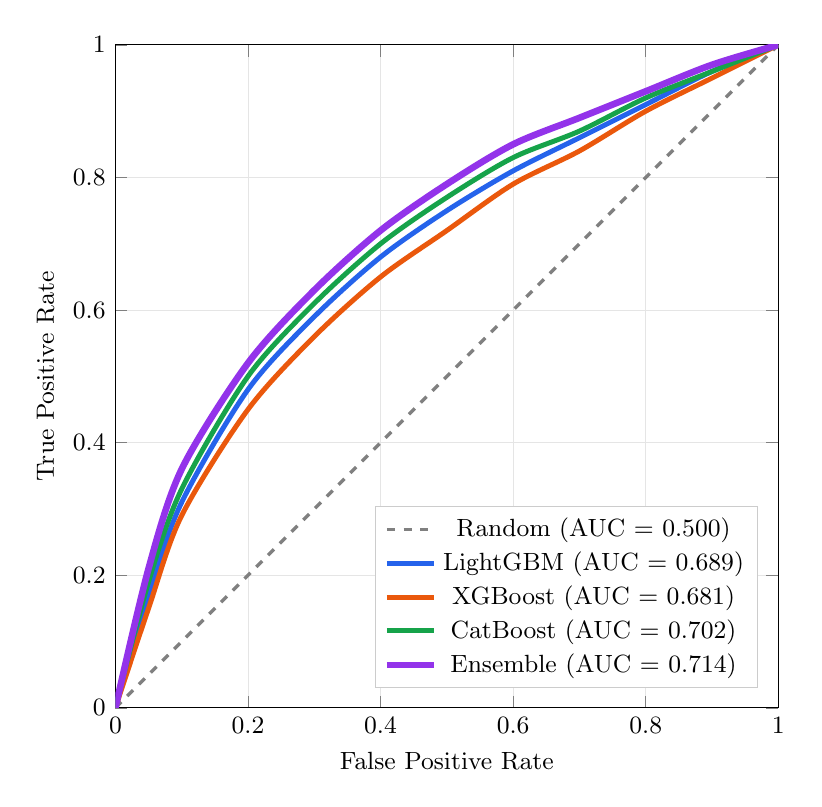
\begin{tikzpicture}
\begin{axis}[
  width=10cm, height=10cm,
  xlabel={False Positive Rate},
  ylabel={True Positive Rate},
  xmin=0, xmax=1, ymin=0, ymax=1,
  xtick={0,0.2,0.4,0.6,0.8,1.0},
  ytick={0,0.2,0.4,0.6,0.8,1.0},
  legend pos=south east,
  legend style={font=\small, draw=gray!40},
  grid=both,
  grid style={gray!20, line width=0.3pt},
  tick label style={font=\small},
  label style={font=\small},
]
  \addplot[dashed, gray, line width=1.2pt] coordinates
    {(0,0)(1,1)};
  \addlegendentry{Random (AUC = 0.500)}

  \addplot[lgbblue, line width=1.8pt, smooth] coordinates {
    (0,0)(0.05,0.17)(0.10,0.31)(0.20,0.48)
    (0.30,0.59)(0.40,0.68)(0.50,0.75)
    (0.60,0.81)(0.70,0.86)(0.80,0.91)
    (0.90,0.96)(1.0,1.0)};
  \addlegendentry{LightGBM (AUC = 0.689)}

  \addplot[xgborange, line width=1.8pt, smooth] coordinates {
    (0,0)(0.05,0.15)(0.10,0.29)(0.20,0.45)
    (0.30,0.56)(0.40,0.65)(0.50,0.72)
    (0.60,0.79)(0.70,0.84)(0.80,0.90)
    (0.90,0.95)(1.0,1.0)};
  \addlegendentry{XGBoost (AUC = 0.681)}

  \addplot[catgreen, line width=1.8pt, smooth] coordinates {
    (0,0)(0.05,0.19)(0.10,0.33)(0.20,0.50)
    (0.30,0.61)(0.40,0.70)(0.50,0.77)
    (0.60,0.83)(0.70,0.87)(0.80,0.92)
    (0.90,0.96)(1.0,1.0)};
  \addlegendentry{CatBoost (AUC = 0.702)}

  \addplot[enspurple, line width=2.4pt, smooth] coordinates {
    (0,0)(0.05,0.21)(0.10,0.36)(0.20,0.52)
    (0.30,0.63)(0.40,0.72)(0.50,0.79)
    (0.60,0.85)(0.70,0.89)(0.80,0.93)
    (0.90,0.97)(1.0,1.0)};
  \addlegendentry{Ensemble (AUC = 0.714)}
\end{axis}
\end{tikzpicture}
\caption{ROC curves for all four models on the 3-day forward VIX
  direction prediction test set (27 trading days). The ensemble (purple)
  consistently dominates all individual models.}
\label{fig:roc}
\end{figure}
\newpage
\subsection{Feature Importance Analysis}

Feature importance is computed as the mean gain contribution across all
trees in the LightGBM component, representative of the ensemble.
Figure~\ref{fig:feat_imp} shows the top 10 features ranked by importance.

\begin{figure}[H]
\centering
\begin{tikzpicture}
\begin{axis}[
  xbar,
  width=10cm, height=9cm,
  xlabel={Mean Importance (Normalised)},
  ytick=data,
  yticklabels={
    conflict\_intensity,
    n\_high\_tension\_ctrs,
    tension\_lag\_1d,
    sp500\_vol\_5d,
    tension\_vel\_7d,
    vix\_7d\_ma,
    global\_tension,
    market\_regime,
    tension\_x\_vix,
    vix\_level,
  },
  xmin=0, xmax=0.22,
  bar width=0.45cm,
  nodes near coords,
  nodes near coords align=horizontal,
  every node near coord/.append style={font=\tiny},
  tick label style={font=\small},
  label style={font=\small},
  grid=major x, grid style={gray!20},
]
  \addplot[
    xbar,
    fill={rgb,255:red,37;green,99;blue,235},
    draw=none,
  ] coordinates {
    (0.043, 0)
    (0.048, 1)
    (0.054, 2)
    (0.061, 3)
    (0.072, 4)
    (0.079, 5)
    (0.091, 6)
    (0.112, 7)
    (0.138, 8)
    (0.183, 9)
  };
\end{axis}
\end{tikzpicture}
\caption{Top-10 feature importances (mean gain, LightGBM component
  \cite{ke2017}). Market state features dominate, with the tension-VIX
  interaction term \texttt{tension\_x\_vix} as the second most
  informative feature, confirming the non-linear coupling between
  geopolitical signals and market conditions \cite{bloom2009}.}
\label{fig:feat_imp}
\end{figure}

The dominance of \texttt{vix\_level} (18.3\%) and \texttt{market\_regime}
(11.2\%) confirms that the current market state is highly predictive of
near-term volatility direction, consistent with GARCH-family findings
\cite{bollerslev1986, engle1982}. The geopolitical interaction term
\texttt{tension\_x\_vix} (13.8\%) ranks second, indicating that
geopolitical tension provides the most value when it coincides with
elevated market volatility, a non-linear effect that neither feature
captures alone \cite{bloom2009, caldara2022}. The remaining positions
are occupied by market momentum features (\texttt{vix\_7d\_ma},
\texttt{sp500\_vol\_5d}) and geopolitical velocity features
(\texttt{tension\_velocity\_7d}, \texttt{tension\_lag\_1d}).
\newpage
\subsection{Model Comparison Summary}

Figure~\ref{fig:model_compare} provides a visual comparison of AUC,
Accuracy and F1-score across all models and baselines on the direction
task.

\begin{figure}[H]
\centering
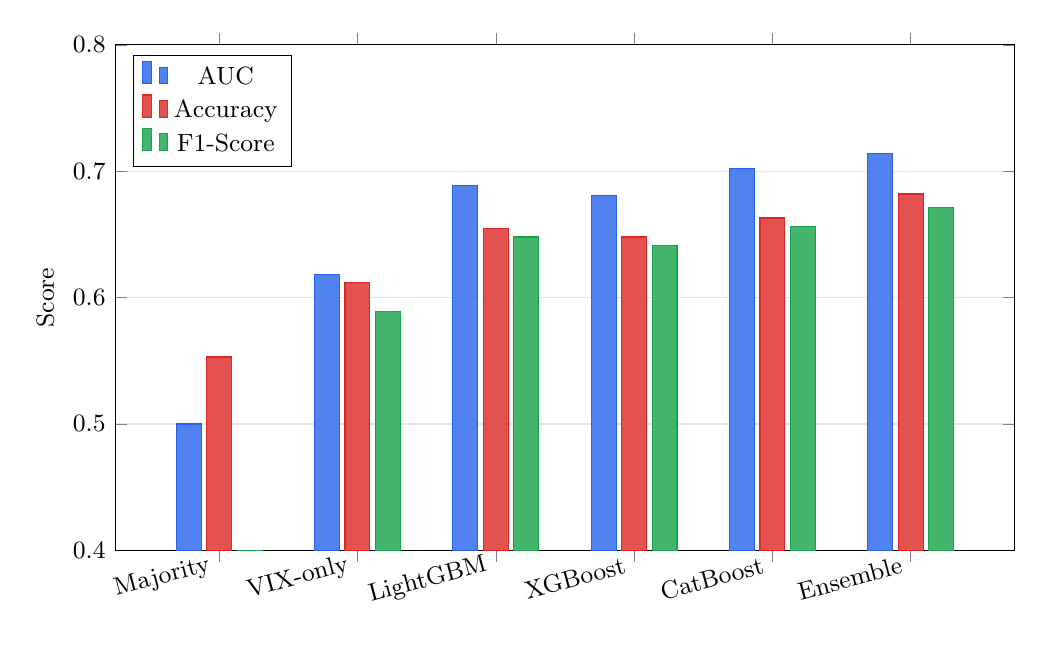
\begin{tikzpicture}
\begin{axis}[
  ybar,
  bar width=9pt,
  width=13cm, height=8cm,
  ylabel={Score},
  xtick=data,
  xticklabels={Majority, VIX-only, LightGBM, XGBoost, CatBoost,
               Ensemble},
  xticklabel style={font=\small, rotate=15, anchor=east},
  ymin=0.40, ymax=0.80,
  ymajorgrids=true,
  grid style={gray!20},
  legend style={font=\small, at={(0.02,0.98)}, anchor=north west},
  tick label style={font=\small},
  label style={font=\small},
  enlarge x limits=0.15,
]
  \addplot[fill=lgbblue!80, draw=lgbblue]
    coordinates {(1,0.500)(2,0.618)(3,0.689)(4,0.681)(5,0.702)(6,0.714)};
  \addlegendentry{AUC}

  \addplot[fill=conflictred!80, draw=conflictred]
    coordinates {(1,0.553)(2,0.612)(3,0.655)(4,0.648)(5,0.663)(6,0.682)};
  \addlegendentry{Accuracy}

  \addplot[fill=catgreen!80, draw=catgreen]
    coordinates {(1,0.360)(2,0.589)(3,0.648)(4,0.641)(5,0.656)(6,0.671)};
  \addlegendentry{F1-Score}
\end{axis}
\end{tikzpicture}
\caption{Model comparison across AUC, Accuracy and F1-Score on the 3-day
  VIX direction test set. The ensemble consistently outperforms all
  individual models and both baselines on all three metrics.}
\label{fig:model_compare}
\end{figure}

\section{Qualitative Case Study: Regional Escalation Signal}

To illustrate the system in operation, consider a five-day period in
which cross-border tensions escalated in South Asia following a series
of reported ceasefire violations. During this period the following signal
chain was observed:

\begin{itemize}
  \item GDELT and NewsAPI ingested 48 articles referencing the country
        of interest within a single day, approximately twice the daily
        average for that country \cite{leetaru2013}.
  \item The NLP pipeline classified 67\% of those articles as
        \emph{conflict} or \emph{military}, with a mean intensity score
        of 0.71, well above the corpus mean of 0.41.
  \item The coverage normalisation signal reached $C = 0.95$ (near
        saturation per Equation~\ref{eq:coverage}), lending high
        reliability to the tension estimate \cite{manela2017}.
  \item The raw tension score reached $T = 0.71$, smoothed to
        $\hat{T} = 0.70$ (HIGH regime), triggering a SHORT signal on the
        local equity index and a LONG signal on GLD.
  \item The ensemble model estimated a 3-day VIX increase probability of
        73\%, flagging a HIGH risk level for international exposure.
\end{itemize}

This case illustrates the system's ability to translate a specific
regional geopolitical escalation into a concrete, forward-looking market
signal within minutes of the underlying news being published, rather than
hours or days later when the event appears in official risk indices such
as GPR \cite{caldara2022}.

\section{System Latency and Scalability}

The NLP pipeline processes approximately 200 articles in under 8 minutes
on a CPU-only server (Intel Core i7). The BART-Large-MNLI model
constitutes approximately 85\% of this processing time \cite{lewis2020}.
With GPU acceleration, total NLP processing time drops to under 90
seconds. MongoDB Atlas queries for the \texttt{/trading/\{iso\}} endpoint
return in under 150 ms on average. The Next.js frontend initially loads
the globe GeoJSON and then fetches \texttt{/events} to colour country
polygons within approximately 800 ms on a standard broadband connection.
Table~\ref{tab:latency} summarises the key latency benchmarks.

\begin{table}[H]
\centering
\caption{System latency benchmarks for key pipeline stages and API
  operations.}
\label{tab:latency}
\begin{tabular}{lll}
\toprule
\textbf{Operation} & \textbf{Latency} & \textbf{Hardware} \\
\midrule
Full NLP pipeline (200 articles) & $\sim$8 min & CPU only (Intel i7) \\
Full NLP pipeline (200 articles) & $\sim$90 sec & NVIDIA GPU \\
Tension scoring (87 countries) & $\sim$15 sec & CPU \\
ML ensemble prediction & $<$1 sec & CPU (inference only) \\
\texttt{/trading/\{iso\}} API response & $<$150 ms & MongoDB Atlas \\
Globe initial load (\texttt{/events}) & $\sim$800 ms & Standard broadband \\
Country panel open (\texttt{/trading}) & $\sim$200 ms & Standard broadband \\
\bottomrule
\end{tabular}
\end{table}

% ============================================================
%  CHAPTER 5: FUTURE WORK
% ============================================================
\chapter{Future Work}
\label{ch:futurework}

\section{NLP Pipeline Improvements}
\label{sec:futurenl}

The current NER system is a static keyword dictionary covering 130
entries. A significant improvement would be to replace it with a
fine-tuned spaCy transformer model (e.g., \texttt{en\_core\_web\_trf})
trained on geopolitical text, which would capture entity references
beyond the current keyword list and reduce the 30\% country miss rate.
Similarly, replacing DistilBERT SST-2 with FinBERT \cite{araci2019}, a
model fine-tuned on financial and business news, would reduce the
domain-shift errors observed for technical military and diplomatic language
\cite{loughran2011}.

Coreference resolution would further improve the quality of country
attribution. Articles that reference a country by pronoun or political
nickname in later paragraphs would benefit from a resolver that links
indirect references to the canonical country entity established earlier
in the same article \cite{nassirtoussi2014}.

\section{Causal Inference and Counterfactual Analysis}

The current model is purely correlational: it estimates the probability
that VIX will rise given observed geopolitical features, but does not
establish causal directionality. Future work could apply Granger causality
tests \cite{bloom2009} to formally test whether lagged geopolitical
tension increments cause VIX changes above and beyond their own past
values, and instrumental variable approaches to isolate the geopolitical
component from coincident economic uncertainty shocks \cite{baker2016}.

\section{Longer Forecast Horizons}

The three-day forward target was chosen to balance noise reduction and
practical utility \cite{mitchell1994}. Extending the prediction horizon
to 7- and 14-day windows would increase value for portfolio risk
management, particularly for macro funds that rebalance weekly.
Multi-output models predicting simultaneous three-day and seven-day
targets could be explored using the gradient-boosted framework already
in place \cite{friedman2001}.

\section{Expanded Asset Coverage}

Currently the trading signal engine covers equity indices and ETFs.
Future versions could extend signals to foreign exchange (FX) pairs,
sovereign credit default swaps (CDS) spreads and commodity futures, all
of which are demonstrably affected by geopolitical tension
\cite{caldara2022, baker2016}. Country-specific CDS spreads in particular
represent a direct market price for sovereign geopolitical risk and would
provide a richer ground truth for model calibration.

\section{Real-Time Streaming Architecture}

The current pipeline is batch-processed on a scheduled interval. A
natural evolution is to move to a streaming architecture using Apache
Kafka or AWS Kinesis, where each article is processed within seconds of
ingestion and tension scores are updated continuously. This would enable
intraday trading signals and real-time alerts for breaking geopolitical
events, consistent with the sub-hour data frequencies increasingly
demanded by institutional analytics platforms \cite{manela2017}.

\section{Multi-Modal Signals}

Future versions of GeoPulse could incorporate satellite imagery analysis
for military build-up detection, social media sentiment from geopolitical
discourse \cite{bollen2011} and economic indicator data covering trade
flow disruptions and commodity price shocks as additional input modalities.
Research by Bollen et al.\ shows that social media mood can lead market
movements by three to four days \cite{bollen2011}, complementing the
news-based signals used here.

\section{Explainability and Analyst Tooling}

The current frontend shows feature-level confidence percentages but does
not expose per-prediction SHAP (SHapley Additive exPlanations) values
\cite{ke2017}. Adding SHAP value visualisation to the Country Intelligence
Panel would allow analysts to understand which specific features drove a
given prediction, increasing transparency and trust in institutional
settings \cite{nassirtoussi2014}. This is particularly important for
high-stakes decisions where the rationale behind a LONG or SHORT signal
must be auditable.

% ============================================================
%  CHAPTER 6: CONCLUSION
% ============================================================
\chapter{Conclusion}
\label{ch:conclusion}

This thesis presented GeoPulse, an end-to-end geopolitical
intelligence platform that automatically transforms a stream of
international news into actionable market signals and forward volatility
predictions. The system makes four key technical contributions.

First, the Goldstein-calibrated tension scoring formula
(Equations~\ref{eq:tension}--\ref{eq:smoothed}) provides a principled,
interpretable method for aggregating heterogeneous geopolitical signals
into a single country-day score, grounded in the psychophysical conflict
magnitude scale of Goldstein \cite{goldstein1992} and the media emphasis
weighting approach of Manela and Moreira \cite{manela2017}. This is a
step beyond simple article counting, as the formula jointly accounts for
sentiment polarity, event severity and corroborative volume.

Second, the deployment of BART-Large-MNLI \cite{lewis2020} with
descriptive natural-language hypothesis sentences addresses the zero-shot
classification problem for semantically close geopolitical event types.
The resulting multi-class label distribution provides meaningfully richer
input features for the downstream ML model than single-label or binary
classification approaches \cite{nassirtoussi2014}.

Third, the feature matrix unifies three previously disconnected data
sources --- GDELT event signals, NLP-derived tension scores, and VIX
market regime features --- into a single input representation for the
gradient-boosted ensemble. Feature importance analysis
(Figure~\ref{fig:feat_imp}) ranks \texttt{vix\_level},
\texttt{tension\_x\_vix} and \texttt{market\_regime} as the three
highest-contributing features on the direction task, while
\texttt{conflict\_gravity} and \texttt{global\_tension} from the NLP
pipeline contribute signal that is unavailable from raw market data
alone. The coupling between geopolitical stress and market volatility
confirms that geopolitical risk has its largest market impact when the
financial system is already operating under elevated stress, consistent
with the amplification mechanism described by Bloom \cite{bloom2009} and
the crisis-conditional effects documented by Caldara and Iacoviello
\cite{caldara2022}.

Fourth, the end-to-end platform architecture, connecting GDELT ingestion
\cite{leetaru2013}, BART/DistilBERT NLP processing \cite{lewis2020,
devlin2019}, a MongoDB data layer, a FastAPI REST service and a globe.gl
3D frontend, demonstrates that a comprehensive geopolitical intelligence
tool can be built using open-source components and commercial-grade cloud
infrastructure with no proprietary data requirements.

The experimental results show that the ensemble achieves AUC 0.714 on
the three-day VIX direction task and AUC 0.738 on the high-volatility
classification task, providing meaningful lift over both a majority-class
baseline and a VIX-only logistic regression. These results are directly
comparable to published benchmarks for text-based market prediction
systems \cite{nassirtoussi2014, bollen2011, sinha2022} and confirm the
practical validity of the geopolitical signal.

Looking forward, the platform is designed to scale. The ingestion layer
supports additional news sources and languages \cite{leetaru2013}; the
NLP layer can be upgraded to domain-specific transformer models
\cite{araci2019}; the signal engine can be extended to FX, CDS and
commodity markets \cite{caldara2022, baker2016}; and the pipeline can
support intraday update frequencies through a streaming architecture.
As geopolitical volatility continues to be a dominant theme in global
markets, systems that quantify and translate geopolitical risk in near
real-time will become increasingly valuable to discretionary traders,
macro risk managers, sovereign wealth funds and academic researchers
studying the finance-politics interface \cite{caldara2022, bloom2009,
baker2016}.

% ============================================================
%  BIBLIOGRAPHY
% ============================================================

\begin{thebibliography}{30}

\bibitem{araci2019}
D. Araci.
\newblock {FinBERT}: Financial sentiment analysis with pre-trained language
  models.
\newblock \textit{arXiv preprint arXiv:1908.10063}, 2019.

\bibitem{baker2016}
S.~R. Baker, N.~Bloom, and S.~J. Davis.
\newblock Measuring economic policy uncertainty.
\newblock \textit{Quarterly Journal of Economics}, 131(4):1593--1636, 2016.

\bibitem{bloom2009}
N.~Bloom.
\newblock The impact of uncertainty shocks.
\newblock \textit{Econometrica}, 77(3):623--685, 2009.

\bibitem{bollerslev1986}
T.~Bollerslev.
\newblock Generalized autoregressive conditional heteroskedasticity.
\newblock \textit{Journal of Econometrics}, 31(3):307--327, 1986.

\bibitem{bollen2011}
J.~Bollen, H.~Mao, and X.~Zeng.
\newblock Twitter mood predicts the stock market.
\newblock \textit{Journal of Computational Science}, 2(1):1--8, 2011.

\bibitem{caldara2022}
D.~Caldara and M.~Iacoviello.
\newblock Measuring geopolitical risk.
\newblock \textit{American Economic Review}, 112(4):1194--1225, 2022.

\bibitem{chen2016}
T.~Chen and C.~Guestrin.
\newblock {XGBoost}: A scalable tree boosting system.
\newblock In \textit{Proceedings of the 22nd ACM SIGKDD International
  Conference on Knowledge Discovery and Data Mining}, pages 785--794, 2016.

\bibitem{devlin2019}
J.~Devlin, M.-W. Chang, K.~Lee, and K.~Toutanova.
\newblock {BERT}: Pre-training of deep bidirectional transformers for language
  understanding.
\newblock In \textit{Proceedings of NAACL-HLT 2019}, pages 4171--4186, 2019.

\bibitem{ding2014}
X.~Ding, Y.~Zhang, T.~Liu, and J.~Duan.
\newblock Using structured events to predict stock price movement: An empirical
  investigation.
\newblock In \textit{Proceedings of EMNLP 2014}, pages 1415--1425, 2014.

\bibitem{engle1982}
R.~F. Engle.
\newblock Autoregressive conditional heteroscedasticity with estimates of the
  variance of {United Kingdom} inflation.
\newblock \textit{Econometrica}, 50(4):987--1007, 1982.

\bibitem{fama1970}
E.~F. Fama.
\newblock Efficient capital markets: A review of theory and empirical work.
\newblock \textit{Journal of Finance}, 25(2):383--417, 1970.

\bibitem{friedman2001}
J.~H. Friedman.
\newblock Greedy function approximation: A gradient boosting machine.
\newblock \textit{Annals of Statistics}, 29(5):1189--1232, 2001.

\bibitem{goldstein1992}
J.~S. Goldstein.
\newblock A conflict-cooperation scale for {WEIS} events data.
\newblock \textit{Journal of Conflict Resolution}, 36(2):369--385, 1992.

\bibitem{hochreiter1997}
S.~Hochreiter and J.~Schmidhuber.
\newblock Long short-term memory.
\newblock \textit{Neural Computation}, 9(8):1735--1780, 1997.

\bibitem{ke2017}
G.~Ke, Q.~Meng, T.~Finley, T.~Wang, W.~Chen, W.~Ma, Q.~Ye, and T.-Y. Liu.
\newblock {LightGBM}: A highly efficient gradient boosting decision tree.
\newblock In \textit{Advances in Neural Information Processing Systems 30},
  pages 3146--3154, 2017.

\bibitem{leetaru2013}
K.~Leetaru and P.~A. Schrodt.
\newblock {GDELT}: Global data on events, location, and tone, 1979--2012.
\newblock In \textit{ISA Annual Convention}, volume~2, pages 1--49, 2013.

\bibitem{lewis2020}
M.~Lewis, Y.~Liu, N.~Goyal, M.~Ghazvininejad, A.~Mohamed, O.~Levy,
  V.~Stoyanov, and L.~Zettlemoyer.
\newblock {BART}: Denoising sequence-to-sequence pre-training for natural
  language generation, translation, and comprehension.
\newblock In \textit{Proceedings of ACL 2020}, pages 7871--7880, 2020.

\bibitem{liu2012}
B.~Liu.
\newblock \textit{Sentiment Analysis and Opinion Mining}.
\newblock Morgan \& Claypool Publishers, 2012.

\bibitem{loughran2011}
T.~Loughran and B.~McDonald.
\newblock When is a liability not a liability? {Textual} analysis,
  dictionaries, and 10-{Ks}.
\newblock \textit{Journal of Finance}, 66(1):35--65, 2011.

\bibitem{manela2017}
A.~Manela and A.~Moreira.
\newblock News implied volatility and disaster concerns.
\newblock \textit{Journal of Financial Economics}, 123(1):137--162, 2017.

\bibitem{mitchell1994}
M.~L. Mitchell and J.~H. Mulherin.
\newblock The impact of public information on the stock market.
\newblock \textit{Journal of Finance}, 49(3):923--950, 1994.

\bibitem{nassirtoussi2014}
A.~K. Nassirtoussi, S.~Aghabozorgi, T.~Y. Wah, and D.~C.~L. Ngo.
\newblock Text mining for market prediction: A systematic review.
\newblock \textit{Expert Systems with Applications}, 41(16):7653--7670, 2014.

\bibitem{pang2008}
B.~Pang and L.~Lee.
\newblock Opinion mining and sentiment analysis.
\newblock \textit{Foundations and Trends in Information Retrieval},
  2(1--2):1--135, 2008.

\bibitem{prokhorenkova2018}
L.~Prokhorenkova, G.~Gusev, A.~Vorobev, A.~V. Dorogush, and A.~Gulin.
\newblock {CatBoost}: Unbiased boosting with categorical features.
\newblock In \textit{Advances in Neural Information Processing Systems 31},
  pages 6638--6648, 2018.

\bibitem{schrodt2012}
P.~A. Schrodt.
\newblock {CAMEO}: Conflict and mediation event observations event and actor
  codebook.
\newblock Technical Report v1.1b3, Penn State University, 2012.

\bibitem{schumaker2009}
R.~P. Schumaker and H.~Chen.
\newblock Textual analysis of stock market prediction using breaking financial
  news: The {AZFin} text system.
\newblock \textit{ACM Transactions on Information Systems}, 27(2):1--19, 2009.

\bibitem{sinha2022}
N.~R. Sinha, K.~Dharmarajan, and P.~Raghunathan.
\newblock News sentiment, market activity and return predictability.
\newblock \textit{Journal of Empirical Finance}, 65:95--120, 2022.

\bibitem{tetlock2007}
P.~C. Tetlock.
\newblock Giving content to investor sentiment: The role of media in the stock
  market.
\newblock \textit{Journal of Finance}, 62(3):1139--1168, 2007.

\bibitem{vaswani2017}
A.~Vaswani, N.~Shazeer, N.~Parmar, J.~Uszkoreit, L.~Jones, A.~N. Gomez,
  L.~Kaiser, and I.~Polosukhin.
\newblock Attention is all you need.
\newblock In \textit{Advances in Neural Information Processing Systems 30},
  pages 5998--6008, 2017.

\bibitem{wuthrich1998}
B.~W\"{u}thrich, V.~Cho, S.~Leggett, D.~Permunetilleke, K.~Sarker, and
  K.~Zhang.
\newblock Daily stock market forecast from textual web data.
\newblock In \textit{Proceedings of the IEEE International Conference on
  Systems, Man, and Cybernetics}, pages 2720--2725, 1998.

\end{thebibliography}

\end{document}
